\todo[inline]{Talk about some motivation for this method: Believe that
  MC does an OK job at estimating fake taus -- no deviations visible
  without corrections. Absence of a good ttbar control region that is
  close to hadhad in the final state -- need to go to lephad for
  measurement.}

\todo[inline]{Maybe say a thing about fake rates for quark / gluon jets.}

\todo[inline]{\tauhadvis misidentification efficiencies should be jet
  misidentification efficiencies in \ttbar.}

A significant background contribution in the \hadhad channel is
represented by \ttbar production where at least one \tauhadvis
candidate is originating from a misidentified quark or gluon
jet. Frequently, this background arises
from~$\ttbar \ra \Pbottom \PWp \APbottom \PWm$ where one \PW boson
decays leptonically producing a real \tauhad and the other decaying
hadronically into jets with one mimicking the signature of a
\tauhadvis in the detector. In this case, hereafter referred to as
semi-leptonic \ttbar, only one \tauhadvis candidate is originating
from a jet and is the dominant source of \faketauhadvis background
from \ttbar in the \hadhad channel. The case where both \tauhadvis
candidates are originating from misidentified jets is comparatively
small explaining approximately~\SI{15}{\percent} of \ttbar with
\faketauhadvis in the signal region of the \hadhad channel. This is
different from the multi-jet background discussed
in~\Cref{sec:hadhad_multijet} where both \tauhadvis candidates are
originating from quark or gluon jets.

\todo[inline]{Clarify that we refer to di-leptonic \ttbar as ttbar
  where both Ws decay leptonically. in semi-leptonic \ttbar only one
  of the W bosons decays leptonically the other hadronically.}

The quality of the modelling of \faketauhadvis in simulation is
generally unknown and no calibrations of selection efficiencies are
provided. The pre-fit distributions shown
in~\Cref{reference}\todo{Find good plots. Maybe 2-tag SS?} show no
indication of large mismodelling of the \faketauhadvis contribution in
simulated \ttbar. A data-driven estimation method is still useful to
provide information about the level of agreement between data and
simulation and to provide uncertainties on these background
contributions.

Given the observed agreement of the Monte Carlo simulation with the
data, an approach of correcting the misidentification efficiencies in
simulation using a data-driven measurement is chosen. Two approaches
were investigated, one being the direct measurement of the
misidentification efficiency in data (the so-called \textit{fake
  rate})
\begin{align*}
  \varepsilon_\text{mis-ID}^\text{data} = \frac{N_\text{post-ID}^\text{data}}{N_\text{pre-ID}^\text{data}}
\end{align*}
and the other being a measurement of the misidentification efficiency
relative to the one in simulation
\begin{align*}
  \text{Fake scale factor:}\quad
  \text{SF} =
  \frac{\varepsilon_\text{mis-ID}^\text{data}}{\varepsilon_\text{mis-ID}^\text{MC}} =
  \frac{N_\text{post-ID}^\text{data} / N_\text{pre-ID}^\text{data}}{N_\text{post-ID}^\text{MC} / N_\text{pre-ID}^\text{MC}}
  = \frac{N_\text{post-ID}^\text{data}}{N_\text{post-ID}^\text{MC}} \cdot \frac{N_\text{pre-ID}^\text{MC}}{N_\text{pre-ID}^\text{data}}
\end{align*}
The second term is completely independent of the modelling of the
\tauhadvis identification efficiency and describes the overall
modelling of \ttbar in Monte Carlo simulation. This term is assumed to
be a constant overall normalisation difference between MC and
data. Differential shape differences will be accounted for in the
systematic uncertainties on \ttbar modelling when extracting the scale
factors.

The correction can be determined including its dependence of
\faketauhadvis properties by performing a maximum likelihood fit in a
dedicated control region enhanced in \ttbar. It can be applied as a
multiplicative factor on \faketauhadvis candidates after \tauhadvis
reconstruction and identification in the \hadhad signal region to
obtain a background estimate. Therefore, it will be called the
\faketauhadvis scale factor (SF) in the following.

\todo[inline]{How would these (fake rates / SFs) be applied any
  differently? What are the advantages of either method?}

\subsubsection{Measurement region}

A top control region is defined in a $\Plepton + \tauhadvis$ final
state with \Plepton being either an electron or a muon. The region is
similar to the top control region used in the \lephad channel where it
is used to calculate fake factors for \tauhadvis mimicked by jets
produced in \ttbar (c.f.\ \cref{sec:}). Minor alterations are applied
to the region definition to ensure a consistent \tauhadvis selection
with the \hadhad channel.

The region is defined by requiring exactly one \tauhadvis passing
loose identification, exactly one electron or muon passing the
identification criteria\todo{reference}, and exactly two \btagged
jets. Only events passing the single lepton trigger selection are
considered. The \tauhadvis and the electron / muon are required to
have opposite electric charge. The \tauhadvis selection is adapted to
more closely follow the selection of the \hadhad channel\footnote{In
  the \lephad channel the \tauhadvis candidates are required to fulfil
  $\pT > \SI{20}{\GeV}$ and $|\eta| < 2.3$.}, that is the \tauhadvis
candidate is required to have $\pT > \SI{25}{\GeV}$ with a
pseudorapidity up to~$|\eta| < 2.5$. Orthogonality with the signal
region of the \lephad channel is ensured by requiring
$\mBB > \SI{150}{\GeV}$.

\todo[inline]{Why OS? SS will likely be enhanced in fakes. Charge
  correlations are more similar to the hadhad SR where the dominant
  contribution are events where only one tau is fake.}

The control region selects \ttbar with high purity of approximately
\SI{94}{\percent} (pre-fit). The largest part, with a purity of
\SI{66}{\percent}, is \ttbar with a $\ell + \tau$ final state where
$\ell$ is either an electron or muon and the $\tau$~lepton decays
hadronically. This contribution will be subsequently referred to as
di-leptonic \ttbar. The production of \ttbar with \tauhadvis
originating from quark or gluon jets, which is the process of interest
for this measurement, constitutes a purity of~\SI{28}{\percent}.
Minor backgrounds in this region are single top (\SI{4}{\percent}) and
vector boson production in association with jets
(\SI{2}{\percent}). The contribution of multi-jet background is
assumed to be negligible.\todo{Why is this negligible? Based on the
  assumptions made by lephad?}

\todo[inline]{Fraction of quark / gluon jets?}


The misidentification efficiencies of jets as \tauhadvis depend on the
identification requirements placed on \tauhadvis candidates during
offline event reconstruction. In this analysis the loose working point
of the RNN \tauhadvis~identification algorithm serves as the baseline
\tauhadvis selection. In the \hadhad channel events are selected with
single- and di-\tauhadvis triggers which use isolation and
identification criteria to reduce trigger-rates in various stages of
the ATLAS trigger system. Calorimeter-based isolation requirements are
applied to \tauhadvis candidates at L1, while at the HLT more
sophisticated \tauhadvis~identification algorithms are used.  The HLT
algorithms were developed to be similar to their counterparts in the
\tauhadvis reconstruction. However, divergences between the
identification algorithms used at the HLT and in offline \tauhadvis
reconstruction are expected due to limitations in detector read-out
and time budget at the HLT. New developments in offline \tauhadvis
reconstruction and identification during Run~2 data-taking cannot be
retroactively applied leading to additional differences between the
algorithms.

The effect of this two-stage selection of \tauhadvis based on
identification criteria, first at trigger-level and then during
offline event reconstruction, needs to be taken into account when
measuring corrections to the \tauhadvis misidentification
efficiencies. Thus one needs to differentiate between both trigger
categories in the \hadhad channel. In events selected by
single-\tauhadvis triggers it is sufficient for a single \tauhadvis to
pass reconstruction and identification at the HLT. For di-\tauhadvis
triggers both candidates need to fulfil the requirements at the HLT.
The top control region, which uses single electron and muon triggers,
allows the direct estimation of corrections for \tauhadvis without any
requirements at the HLT.

The selection at the HLT can be emulated by requiring that events in
the top control region, which were originally selected using single
lepton triggers, also pass an appropriately chosen single-\tauhadvis
trigger and that the \tauhadvis candidate is matched to a
reconstructed and identified \tauhadvis at the HLT. At HLT-level the
lowest transverse momentum threshold on the \tauhadvis relevant for
this analysis is $\pTHLT > \SI{25}{\GeV}$, with the chain of HLT
algorithms corresponding to the selection employed in the \hadhad
signal region (cf.\ \Cref{sec:exp_trigger}). Generally, only prescaled
versions of these triggers were available during data-taking in Run~2
of the LHC but given that the events are already recorded using single
lepton triggers, the HLT algorithms can be re-run such that these
trigger decisions can be \textit{resurrected} without the application
of a prescale. The relevant single-\tauhadvis triggers are listed in
the following\footnote{For an explanation of the nomenclature see
  \Cref{reference}}:
\begin{itemize}

\item \verb|HLT_tau25_medium1_tracktwo|: Primary trigger chain used
  for data-taking from 2015 to 2017. Resurrected trigger decisions are
  available for the entire Run~2 dataset corresponding to
  \SI{139}{\ifb} of integrated luminosity.

\item \verb|HLT_tau25_medium1_tracktwoEF|: Primary trigger chain used
  for data-taking in 2018. Resurrected trigger decisions are only
  available for runs in 2018 corresponding to an integrated luminosity
  of \SI{58}{\ifb}.

\item \verb|HLT_tau25_mediumRNN_tracktwoMVA|: Supplementary trigger
  chain introduced starting with period K in 2018. The available
  dataset corresponds to \SI{37}{\ifb} of integrated luminosity.  This
  trigger chain is recommended to be used in conjunction with the
  previous item. Hereafter, when refering to
  \verb|HLT_tau25_mediumRNN_tracktwoMVA| a ``logical or'' with
  \verb|HLT_tau25_medium1_tracktwoEF| is implied.

\end{itemize}

In total four configurations of \tauhadvis selection need to be
considered when measuring corrections to the \tauhadvis
misidentification efficiencies in \ttbar. In case of no additional HLT
requirements, these can be determined from the top control region
directly. Three non-disjoint sub-regions of the top control region are
defined for cases where requirements are imposed on \tauhadvis at the
HLT. These are defined by ensuring that the resurrected triggers
select the event and that the reconstructed \tauhadvis candidate is
geometrically matched to the \tauhadvis candidate at the HLT. Separate
measurements are performed in these regions.

\todo[inline]{Talk about offline reconstructed taus and their identification}


\subsubsection{Fit model}

The \tauhadvis misidentification efficiencies strongly depend on the
charged particle multiplicity and visible transverse momentum of the
reconstructed \tauhadvis candidate (c.f.\ \Cref{sec:tauid}). This
might also be reflected in corrections to the misidentification
efficiency of \tauhadvis in simulation. Therefore, the correction
factor measurement is performed in dependence of the reconstructed
decay mode (1- or 3-prong) and \tauhadvis~\pT. This is achieved by
performing a scale factor measurement in disjoint subregions defined
as follows:
\begin{itemize}

\item 1-prong \tauhadvis with $\pT / \si{\GeV}$: $[25, 30)$, $[30, 35)$,
  $[35, 40)$, $[40, 45)$, $[45, 55)$, $[55, 70)$, $[70, \infty)$.

\item 3-prong \tauhadvis with $\pT / \si{\GeV}$: $[25, 30)$, $[30, 40)$,
  $[40, 50)$, $[50, 70)$, $[70, \infty)$.

\end{itemize}
These regions are chosen such that their size allows for a
determination of the corrections with limited impact of statistical
uncertainties while allowing to extract potential \pT dependencies of
the correction factors. In cases where trigger-matching is applied the
\tauhadvis \pT interval from 25 to \SI{30}{\GeV} is omitted due to the
trigger not being fully efficient in this regime. This is analogous to
the selection applied for the \hadhad signal region. An exemplary
summary of the measurement regions is shown
in~\Cref{fig:ttbarsf_region_summary_prefit}.

\begin{figure}[htbp]
  \centering

  \begin{subfigure}[t]{.485\textwidth}
    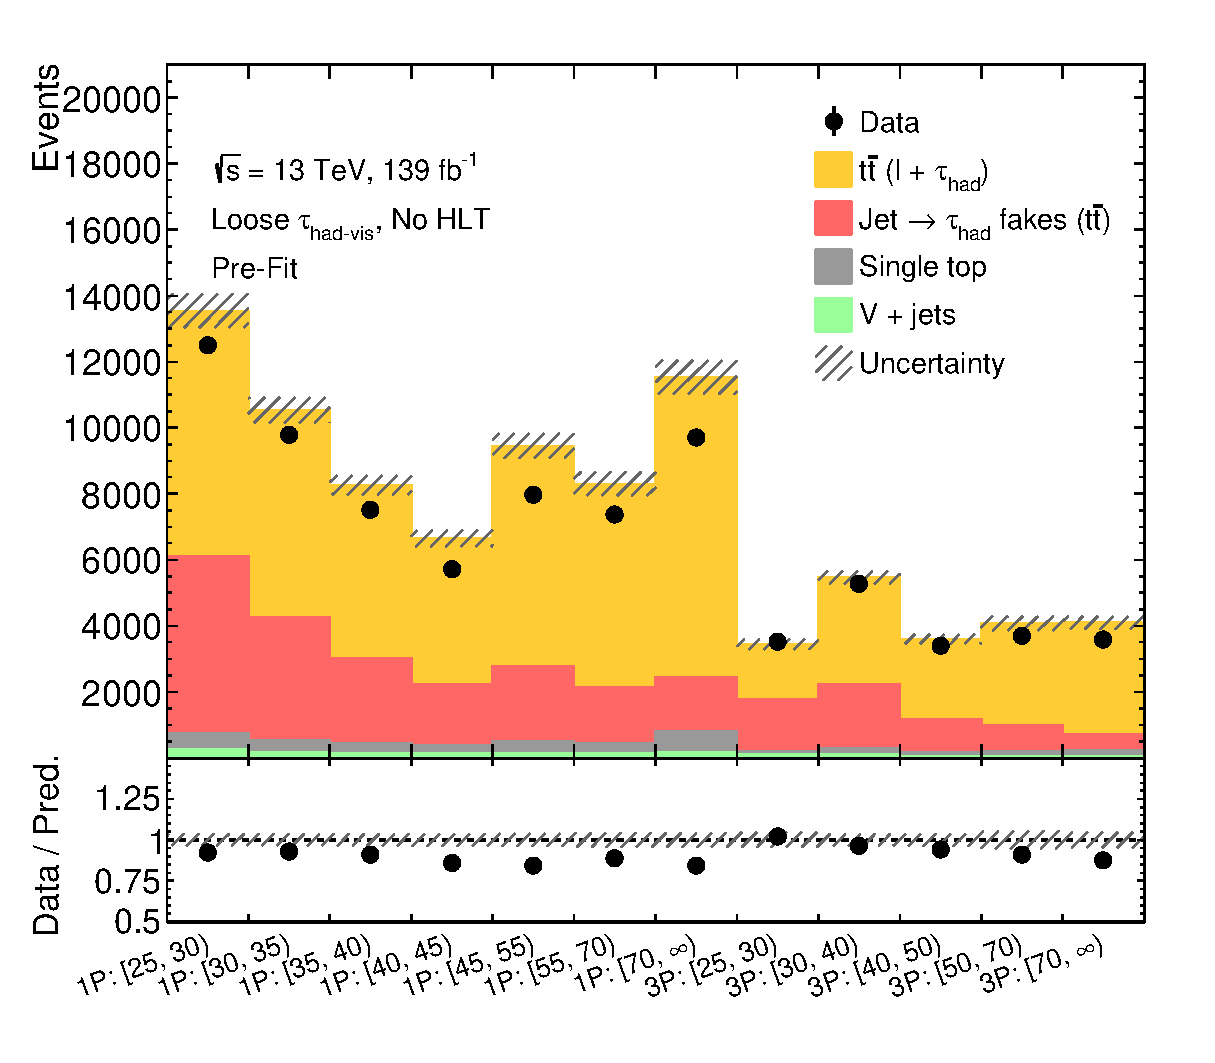
\includegraphics[width=\textwidth]{ttbarSF/Summary_offl}
    \caption{Top control region for events passing the loose
      \tauhadvis identification criteria without trigger-matching.}
  \end{subfigure}\hfill%
  \begin{subfigure}[t]{.485\textwidth}
    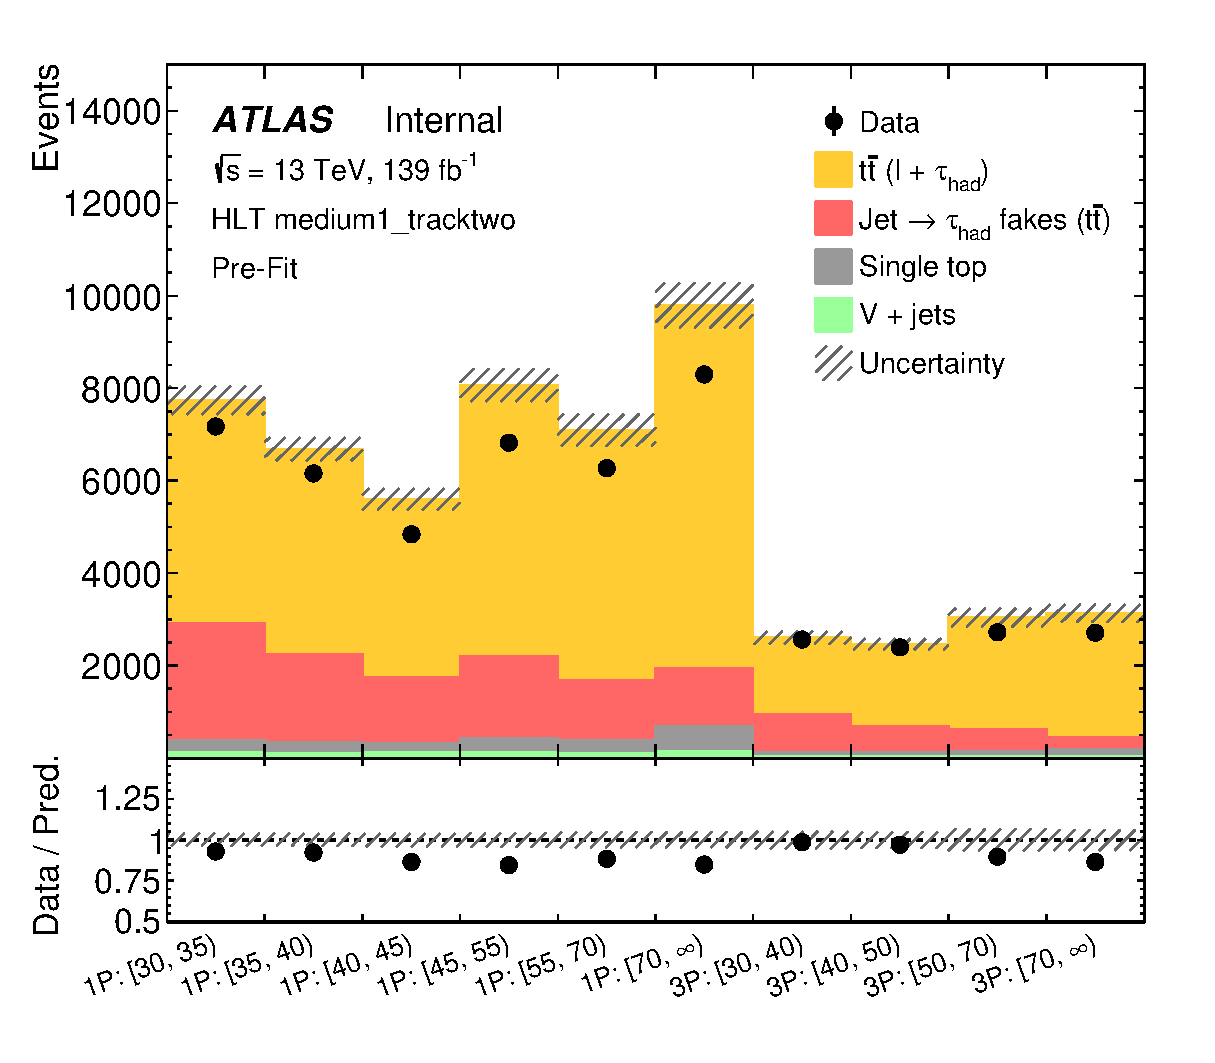
\includegraphics[width=\textwidth]{ttbarSF/Summary_tau25}
    \caption{Top control region for events passing the resurrected
      \texttt{HLT\_tau25\_medium1\_tracktwo} trigger and requiring
      matching between the reconstructed \tauhadvis at HLT and after
      offline \tauhadvis reconstruction.}
  \end{subfigure}

  \caption{Summary of regions used for determination of the \tauhadvis
    misidentification efficiency corrections. The $x$-axis shows the
    regions separated according to the reconstructed decay mode into
    either 1-prong (1P) and 3-prong (3P) \tauhadvis as well as the
    \tauhadvis $\pT /\si{\GeV}$ bin interval. The figures are shown
    with the pre-fit background model.}
  \label{fig:ttbarsf_region_summary_prefit}
\end{figure}

The top control region has a large contamination of \ttbar with a
di-lepton final state where the \tauhadvis candidate originates from a
\tauhad decay. This contribution is not sensitive to the jet \ra
\tauhadvis misidentification efficiency but has to be estimated when
extracting correction factors. To distinguish between di-leptonic
\ttbar with true \tauhadvis and primarily semi-leptonic \ttbar with
\faketauhadvis, an estimate of the transverse mass between the lepton
$\ell$ and \pTmissAbs given by
\begin{align*}
  \mTW = \sqrt{2 | \myvec{p}_{\text{T}}^{\ell} | | \pTmiss | \left( 1 - \cos \Delta\phi \right)}
\end{align*}
is used\footnote{Under the assumption of massless daughter particles
  in a two-body decay.}, where $\Delta \phi$ is the angle between the
lepton transverse momentum~$\myvec{p}_{\text{T}}^{\ell}$ and the
missing transverse momentum~\pTmiss.

The distribution of \mTW for \ttbar with di- and semi-leptonic final
states is shown in~\Cref{fig:ttbarsf_mtw_pdf} for the considered top
control region.
% inclusive in reconstructed \tauhadvis decay mode and transverse momentum.
The primary source of events containing a \faketauhadvis is
semi-leptonic \ttbar with an electron or muon and additional jets from
the hadronic decay of a \PW boson. This contribution features a quick
reduction in event rate for transverse masses beyond the mass of the
\PW boson. In contrast, di-leptonic \ttbar final states show a
comparatively heavy tail towards large values of \mTW due to the
presence of an additional neutrino.  The \mTW distribution of
semi-leptonic \ttbar remains stable with respect to changes in the
considered momentum range for the reconstructed \tauhadvis
candidate. This is not the case for the di-lepton contribution where
the tail towards high \mTW is further enhanced with increasing \pT of
the \tauhadvis candidate\todo{Show?}.

% The main idea is to distinguish between semi-leptonic and di-leptonic
% \ttbar since two true taus would be expected in di-leptonic and jets
% faking taus in semi-leptonic. The all-hadronic mode is negligible due
% to the presence of one electron or muon.

% For semi-leptonic \ttbar the mTW distribution is relatively
% insensitive to the momentum of the tauhadvis candidate. Which is not
% the case for di-leptonic \ttbar.

% For semi-leptonic \ttbar the event rate drops
% significantly beyond \SI{100}{\GeV} while for di-leptonic \ttbar, due
% to the presence of additional neutrinos, the transverse mass extends
% to larger values.

\begin{figure}[htbp]
  \centering

  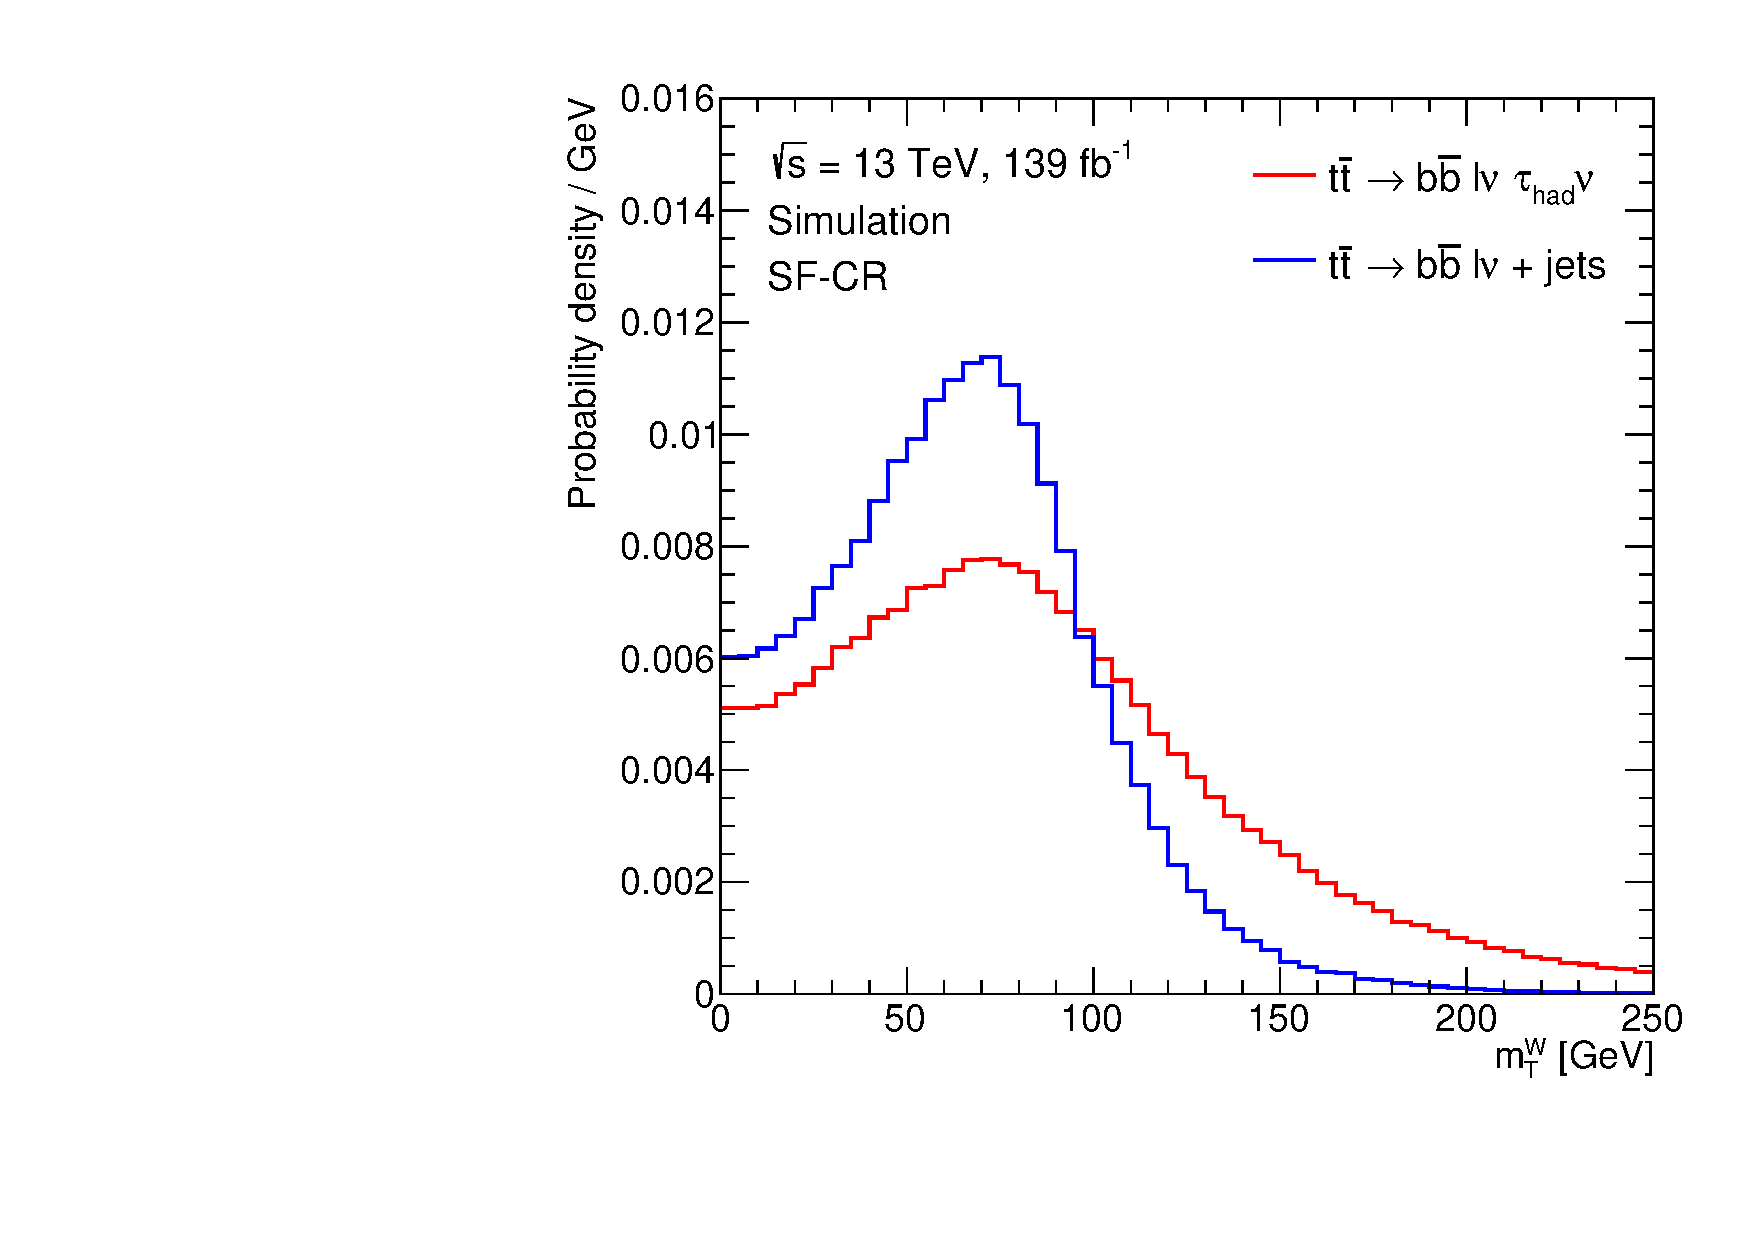
\includegraphics[width=0.45\textwidth]{ttbarSF/mtw_pdf}

  \caption{Transverse mass distribution between lepton and \pTmiss in
    \ttbar simulation. Inclusive in \tauhadvis transverse momentum and
    decay mode. Without applying HLT requirements.}
  \todo[inline]{Missing neutrino for \tauhad?}
  \label{fig:ttbarsf_mtw_pdf}
\end{figure}


% Fit model

% - Top control region (possibly after HLT matching) split um in decay
% mode and \tauhadvis pt bins
% - 5 bins in mTW (40 GeV width) are used to separate the contributions
% - In every bin freely float the fake tauhadvis contribution
% - Globally float the ttbar cross section (affecting both the true and fake tau components)
% -> This is done because at low momenta the separation by mTW

The regions entering the fit model are determined by the charged
particle multiplicity of the reconstructed \tauhadvis candidate and
the reconstructed \tauhadvis \pT. For the measurement after HLT
\tauhadvis identification the events entering the fit are also
required to pass trigger matching to the resurrected trigger of
interest. Each measurement region enters the fit with five bins in
\mTW to distinguish between \ttbar with \faketauhadvis and real
\tauhadvis. In~\Cref{fig:ttbarsf_mtw_examples_prefit} the \mTW
distribution is shown prior to the fit for two exemplary regions after
requiring trigger-matching.  The normalisation of \ttbar with
\faketauhadvis is allowed to vary freely in every measurement region
separately. The total \ttbar cross section is extracted from the fit
to data. This is accomplished by allowing the normalisation of \ttbar
with and without \faketauhadvis to vary freely. The associated
normalisation factor is fully correlated between all measurement
regions. This approach is taken as opposed to leaving the overall
\ttbar cross section free in every sub-region separately due to the
weak discrimination power of \mTW for small \tauhadvis \pT.


\begin{figure}[htbp]
  \centering

  \begin{subfigure}{.485\textwidth}
    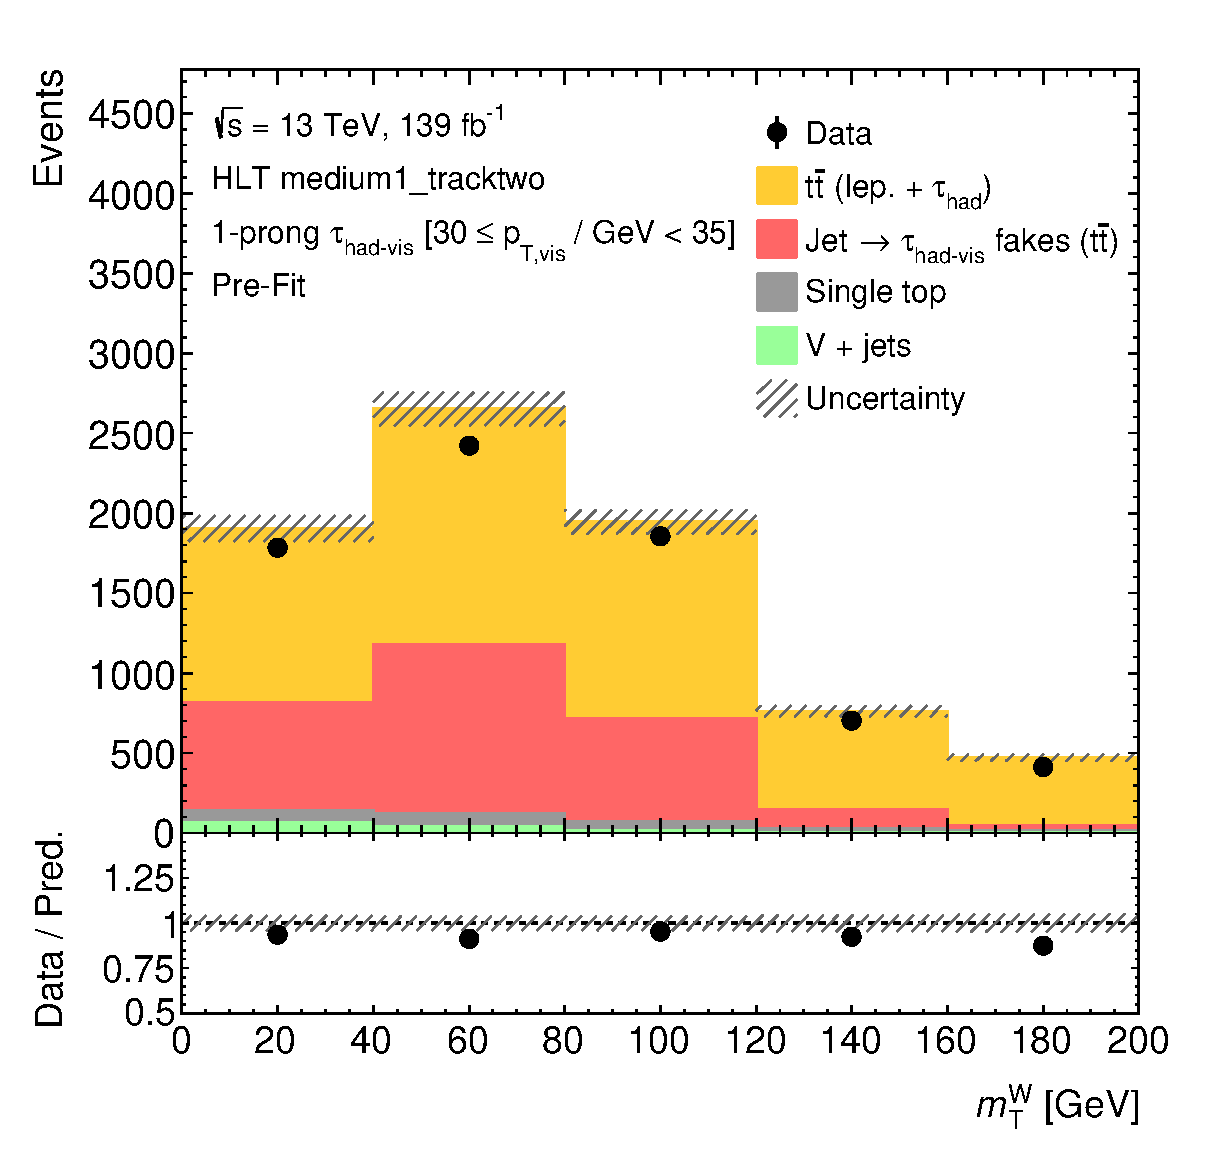
\includegraphics[width=\textwidth]{ttbarSF/tau25/TauPt3035_1P}
    \caption{1-prong \tauhadvis candidates with
      $\SI{30}{\GeV} \leq \pTvis < \SI{35}{\GeV}$.}
  \end{subfigure}\hfill%
  \begin{subfigure}{.485\textwidth}
    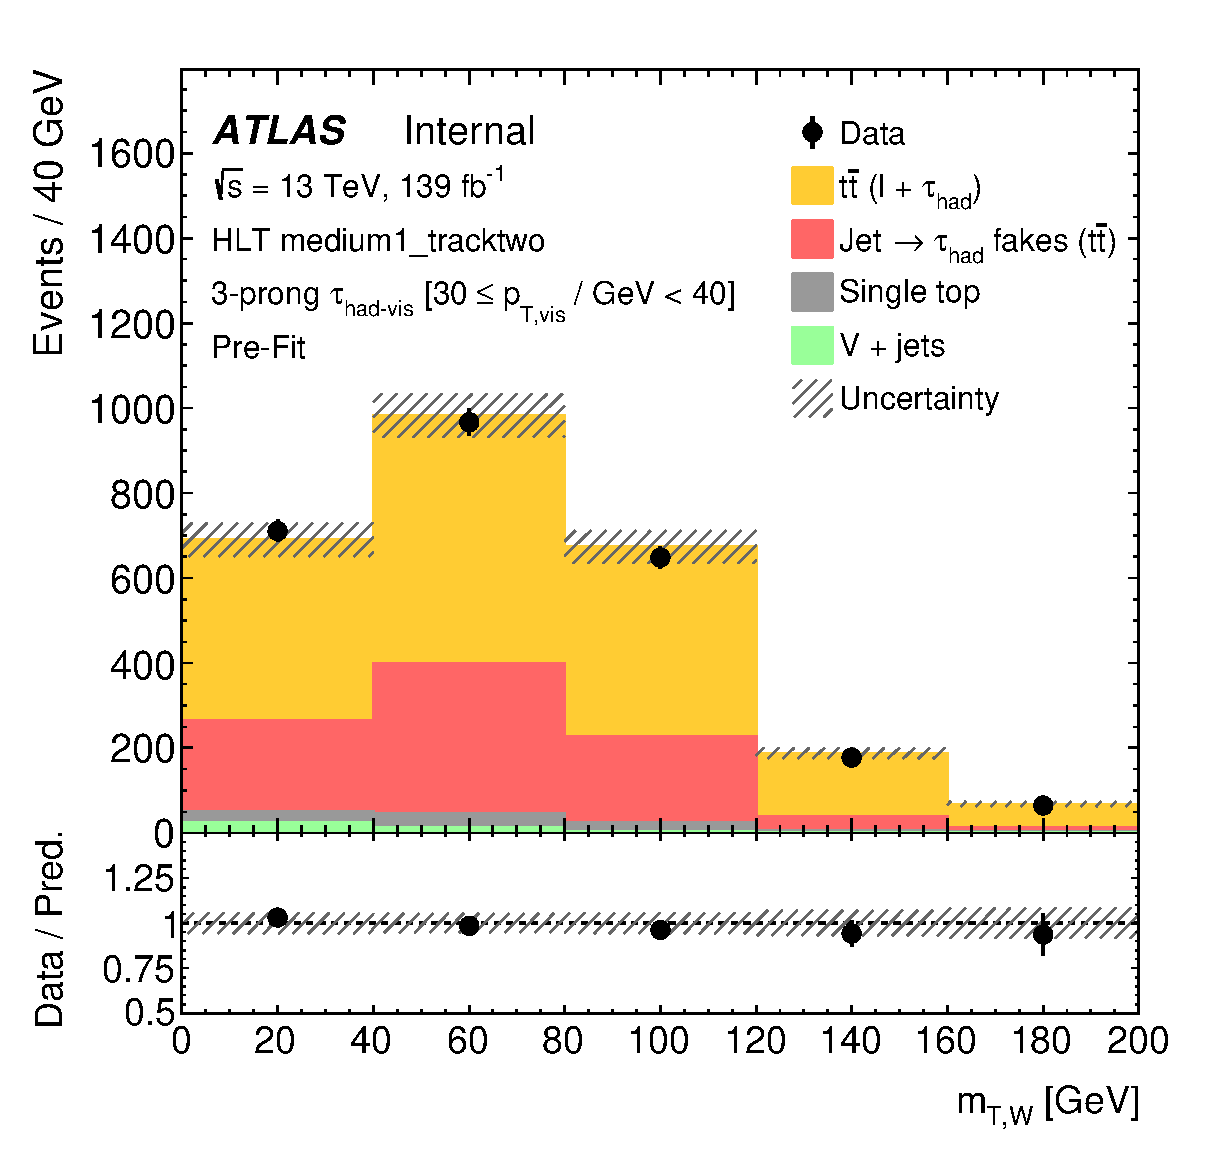
\includegraphics[width=\textwidth]{ttbarSF/tau25/TauPt3040_3P}
    \caption{3-prong \tauhadvis candidates with
      $\SI{30}{\GeV} \leq \pTvis < \SI{40}{\GeV}$.}
  \end{subfigure}

  \caption{Two examples of \mTW distributions. Events with
    $\mTW > \SI{200}{\GeV}$ are merged into the last bin of the
    histogram.}
  \label{fig:ttbarsf_mtw_examples_prefit}
\end{figure}


\subsubsection{Uncertainties}

The expected number of events in bins entering the statistical
analysis are subject to statistical, experimental and theoretical
uncertainties. These uncertainties can affect the shapes and
normalisations of the predictions and the relative acceptance between
different measurement regions. As a result, systematic uncertainties
affecting the modelling of \ttbar with true and fake-\tauhadvis are of
primary concern due to their ability to alter the the extracted scale
factors. In the following a description of the uncertainties is given
with a focus of theoretical modelling uncertainties dedicated to this
measurement. Experimental uncertainties are only briefly summarised
due to their overlap with the uncertainties in the model used to
extract the di-Higgs signal. A more detailed discussion on
experimental uncertainties will follow when discussing this fit model
in~\Cref{sec:uncertainties}.

Statistical uncertainties arising from the finite size of the
simulation used to estimate the physics processes entering this
measurement. These uncertainties are encoded in the likelihood model
using the Barlow-Beeston method~\cite{barlow1993,conway2011}.

Major detector-related experimental uncertainties originate from the
reconstruction and selection of electrons, muons, \tauhadvis and jets.
These uncertainties affect the reconstructed momenta in scale,
resolution and direction as well as the selection efficiencies of
reconstructed objects and events, e.g.~due to isolation requirements
or the trigger selection. When requiring events to pass the
resurrected trigger decision of single \tauhadvis triggers,
calibrations of trigger selection efficiencies and their associated
uncertainties are applied to \tauhadvis that are geometrically matched
to \tauhad. Uncertainties in the reconstruction of the missing
transverse momentum are accounting for changes in momentum scale and
resolution. The uncertainty on efficiencies for \bjets passing \btag
and mis-tag rates of jets originating from light and charm quarks are
propagated from dedicated calibration measurements performed by the
ATLAS collaboration. Other experimental uncertainties originating from
trigger efficiencies of single lepton triggers, efficiency of jet
vertex tagging, reweighting of pile-up conditions in simulation to
match the Run~2 conditions, and the luminosity used to normalise the
simulated datasets are included.

% https://twiki.cern.ch/twiki/bin/viewauth/AtlasProtected/PmgTopProcesses
Theoretical uncertainties on the acceptance of \ttbar in simulation,
which uses \POWHEGBOX[v2]~\cite{Frixione:2007nw} as a matrix element
(ME) generator interfaced to \PYTHIA[8.230]~\cite{Sjostrand:2014zea}
for the parton shower (PS), need to be estimated. The total cross
section of \ttbar is allowed to vary freely in the fit model, thus
uncertainties on the overall normalisation of \ttbar are
omitted. However, uncertainties changing the relative acceptance
between regions entering the simultaneous fit and effects changing the
shape of the \mTW discriminant need to be estimated. The following
sources of uncertainties are considered:
\begin{itemize}

\item Hard scatter and NLO+PS matching: The uncertainty on the
  modelling due to the choice of generator describing the hard scatter
  process is estimated by comparing the nominal simulation of \ttbar
  with an alternative setup replacing \POWHEGBOX[v2] with \MGNLO as
  the ME generator. This comparison serves to probe the effect of
  different matching schemes between the NLO matrix element and parton
  shower employed by both generators (\POWHEG
  method~\cite{Nason:2004rx,Frixione:2007vw,Alioli:2010xd} / MC@NLO
  method~\cite{Frixione:2002ik}).

\item Parton shower and hadronisation model: The uncertainty of the
  modelling of the parton shower and non-perturbative effects is
  estimated by replacing \PYTHIA[8] with \HERWIG[7.0.4] as the PS
  generator.

\item Missing higher order contributions: The renormalisation
  scale~\muR and factorisation scale~\muF is doubled and halved to
  probe the effect of truncating the perturbative expansion in \alphas
  in the simulation of the hard scatter. Perturbative QCD calculations
  at sufficiently high orders should be approximately independent of
  the scales.

\item Initial and final state radiation (ISR \& FSR): An uncertainty
  on the emission of ISR is estimated by varying $\alphas^\text{ISR}$
  in the A14 set of tuned parameters for
  \PYTHIA[8]~\cite{ATL-PHYS-PUB-2014-021}.
  % Tune of the MPI, ISR, FSR parameters in Pythia8
  An estimate of the uncertainty from the modelling of FSR is
  estimated by doubling / halving the renormalisation scale used for
  FSR branchings in \PYTHIA[8].
  % https://pythia.org/latest-manual/Variations.html

\item Damping factor for first emission (NLO+PS matching): The damping
  parameter~\hdamp in \POWHEGBOX[v2] is increased to
  $3 m_\text{top}$ (from $1.5 m_\text{top}$) and compared with the
  nominal simulation setup. The \hdamp parameter effectively
  controls the modelling of the first emission beyond Born-level in
  the NLO+PS \POWHEG-method.
\end{itemize}
% PDF uncertainties were neglected.
The prescriptions to calculate the \ttbar modelling uncertainties are
a revised version of the methodology outlined
in~\cite{ATL-PHYS-PUB-2020-023} for analyses targeting the full Run~2
dataset collected at the ATLAS experiment.

Variations of the renormalisation and factorisation scales used for
the ME generation are provided by internal reweighting in
\POWHEGBOX[v2]. Similarly, \PYTHIA[8] provides variations of initial
and final state emissions by varying the renormalisation scales in the
PS by reweighting~\cite{Mrenna:2016sih}. This approach allows to
estimate uncertainties without changing the particle-level predictions
of the simulation program.

Uncertainties estimated by performing a two-sample comparison (NLO+PS
matching, PS, \hdamp) are parametrised in \tauhadvis \pT,
reconstructed \tauhad decay mode and \mTW separately for \ttbar with
true and \faketauhadvis. A smooth functional dependence of these
uncertainties is obtained by performing polynomial regression of the
relative change in yield comparing the alternative with the nominal
sample in bins of \tauhadvis \pT and \mTW. This approach is taken to
avoid spurious pulls and constraints of the associated nuisance
parameters in the maximum likelihood fit originating from statistical
fluctuations of the derived uncertainties.

In every category, i.e.\ 1-prong / 3-prong \tauhadvis and true- /
\faketauhadvis, ordinary least squares regression is performed for all
three sources of uncertainty. The degree of the fitted polynomials is
determined by leave-one-out cross-validation yielding the lowest
$\chi^2$ with small variance of the $\chi^2$ statistic. As a first
step, the effect of the uncertainty on \tauhadvis \pT is estimated. An
example of this is shown
in~\Cref{fig:ttbarSF_uncertainty_ps_1p_pt,fig:ttbarSF_uncertainty_ps_3p_pt}
for the PS variation.

Subsequently, the nominal sample is reweighted using the estimated
\pT-dependency and the residual non-closure in \mTW is examined. The
non-closure in \mTW is small after taking the \tauhadvis \pT effect of
the variation into account. Minor shape differences are only observed
for the ME and PS generation variations for true \tauhadvis. An
example is shown
in~\Cref{fig:ttbarSF_uncertainty_ps_1p_mtw,fig:ttbarSF_uncertainty_ps_3p_mtw}
for the PS variation. The non-closure is assigned as an uncertainty
fully correlated with the \pT effect. The variations of the damping
parameter related to the NLO+PS matching in \POWHEG show no
statistically significant effect depending on \tauhadvis \pT or
\mTW. Thus only an uncertainty on the relative normalisation between
categories is assigned.

\begin{figure}[htbp]
  \centering

  \begin{subfigure}[t]{.48\textwidth}
    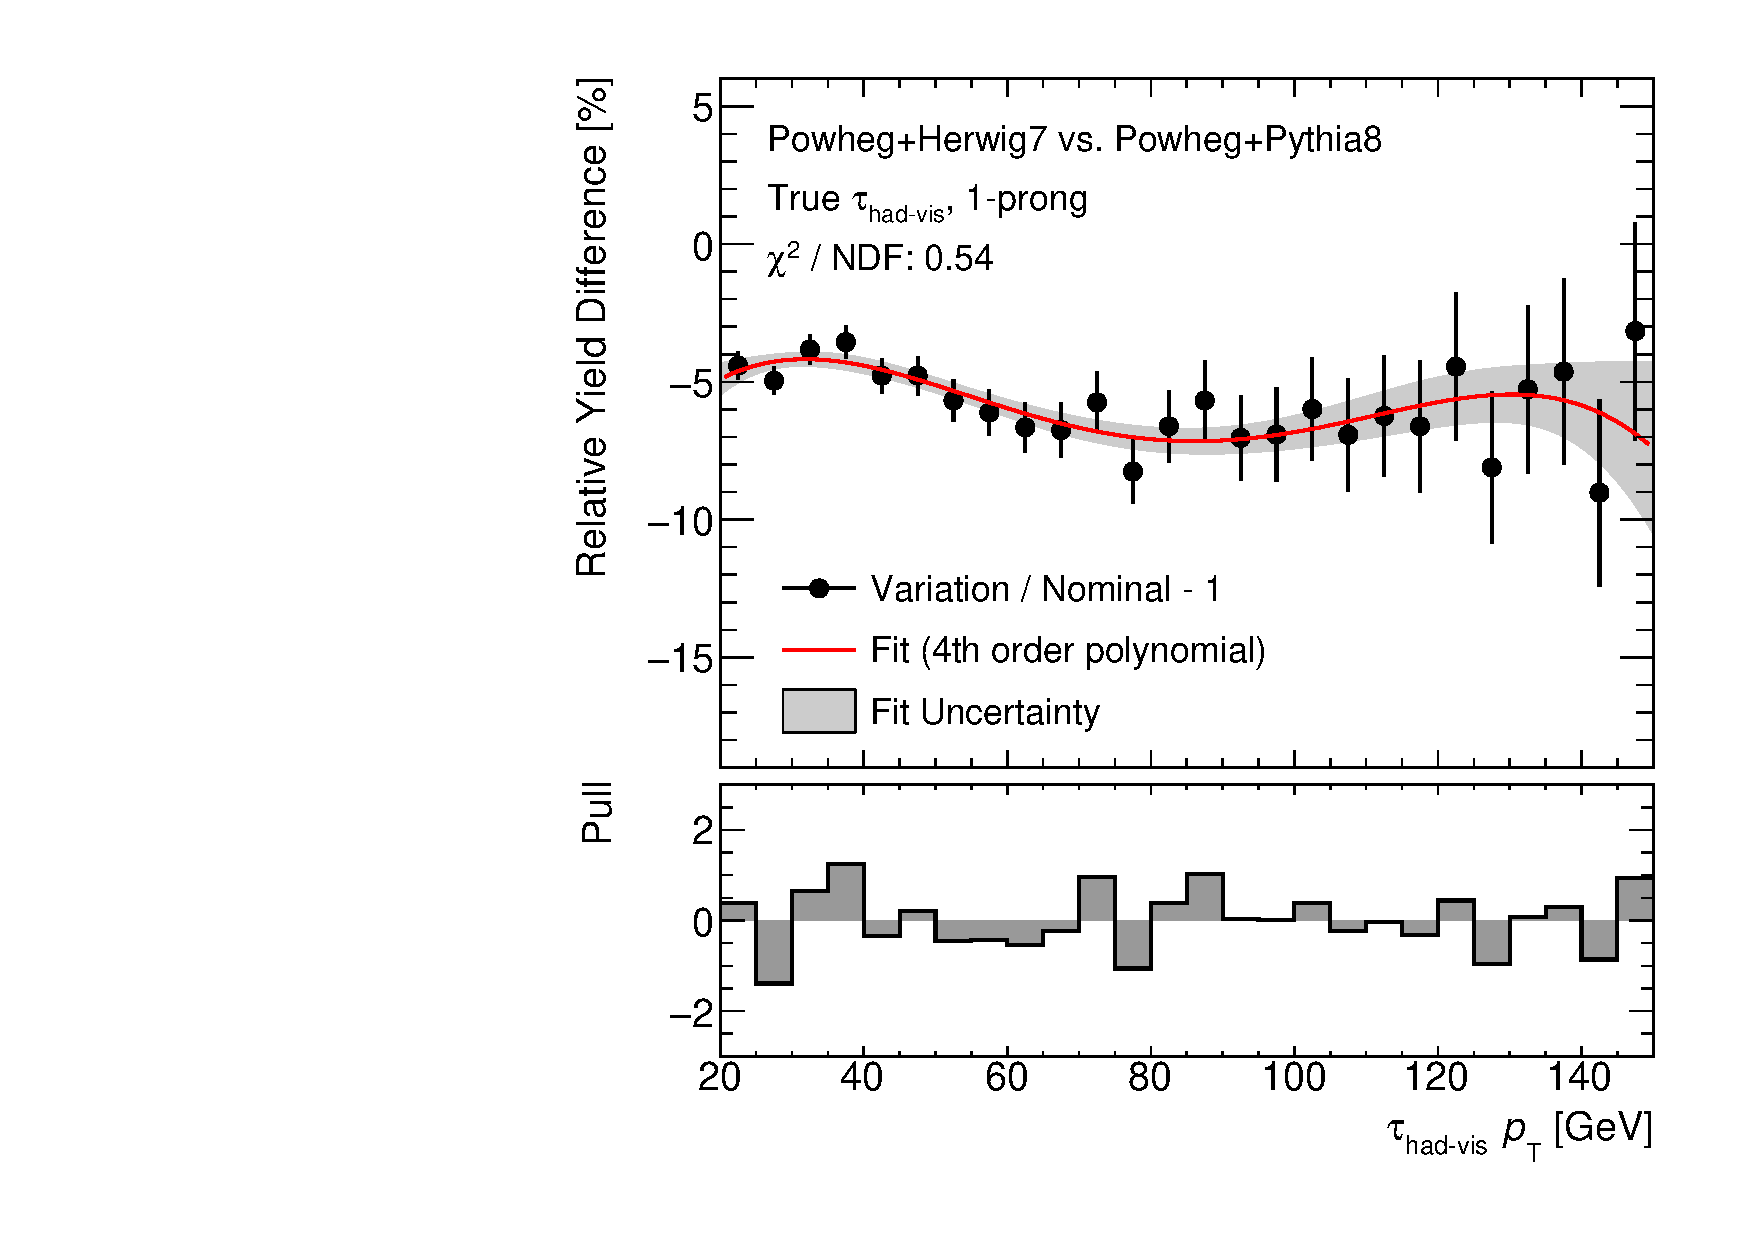
\includegraphics[width=\textwidth]{ttbarSF/uncertainties/ps_true_1p_pt}
    \caption{Impact of the PS variation on \tauhadvis \pT for 1-prong
      \tauhadvis.}
    \label{fig:ttbarSF_uncertainty_ps_1p_pt}
  \end{subfigure}\hfill%
  \begin{subfigure}[t]{.48\textwidth}
    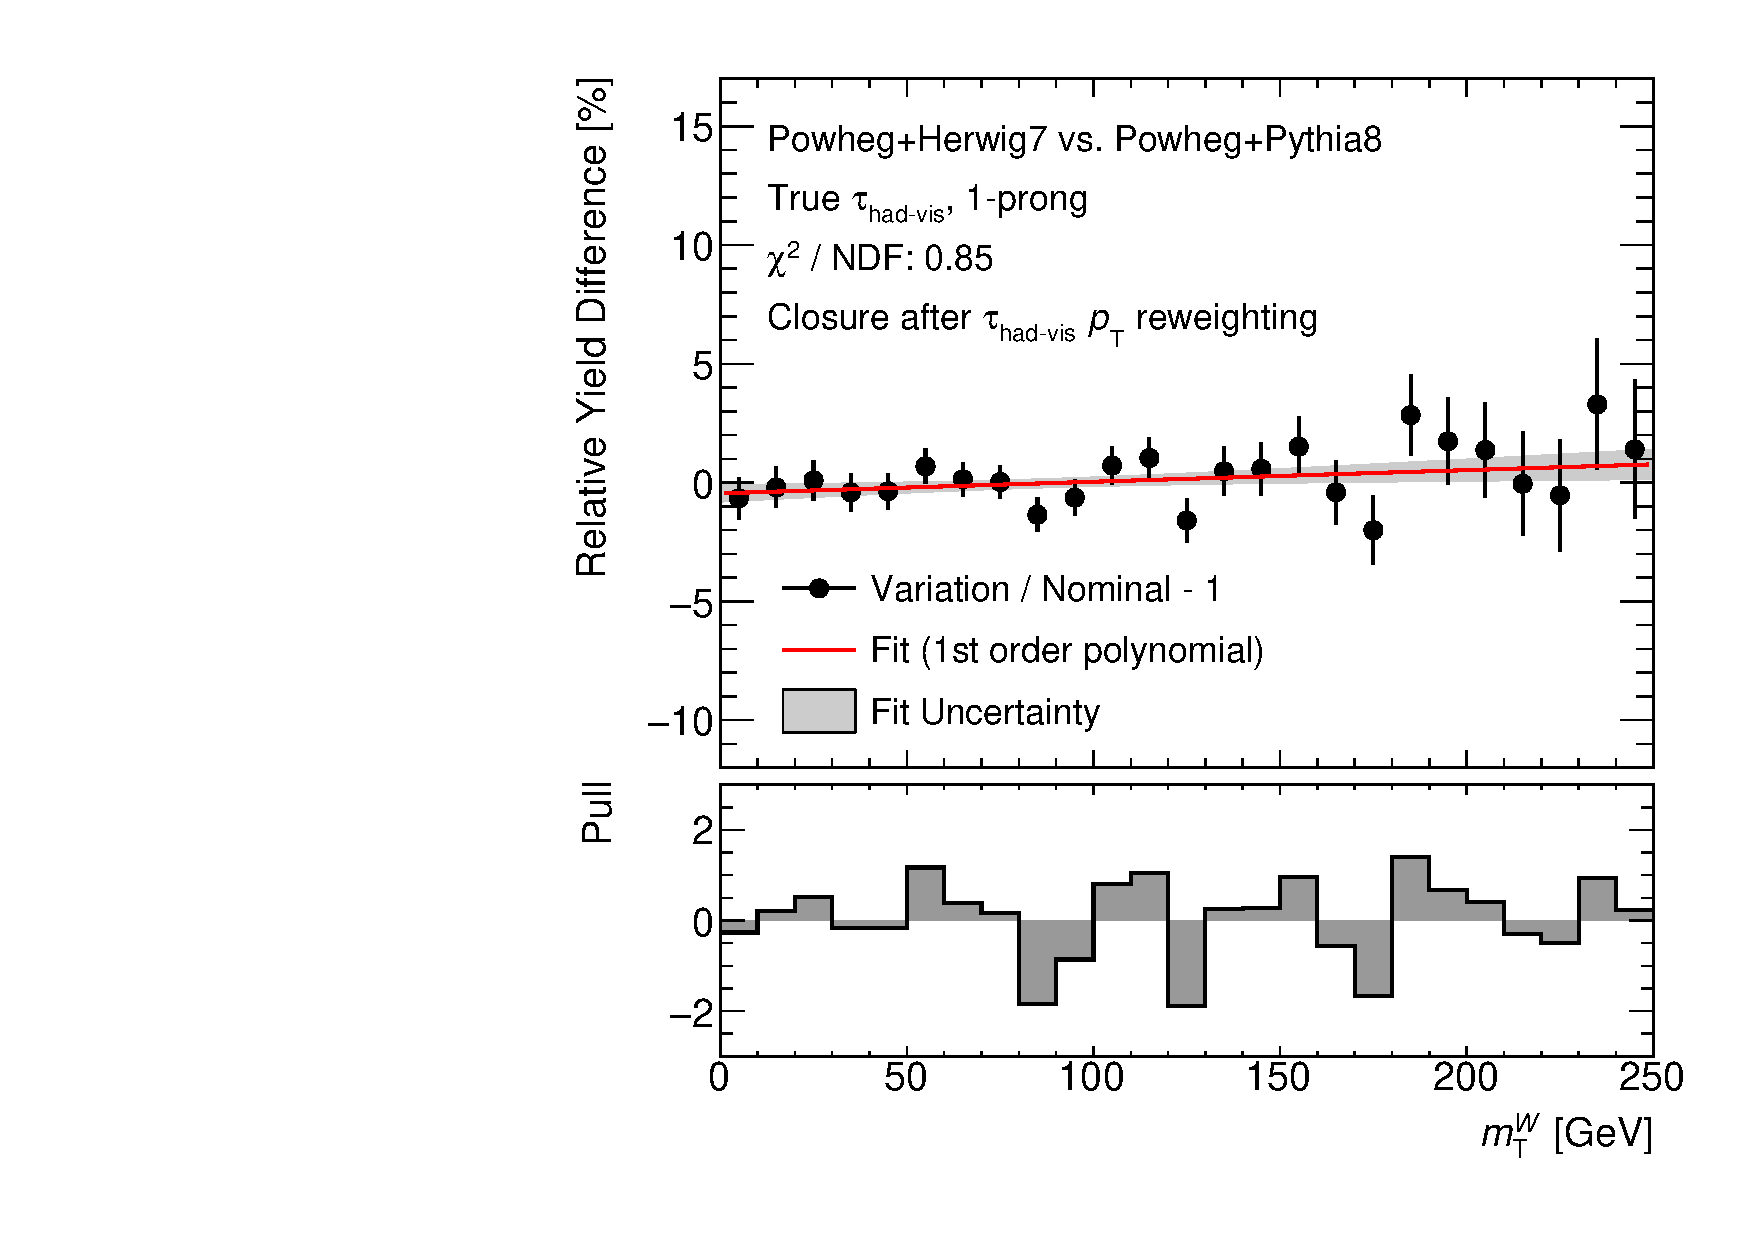
\includegraphics[width=\textwidth]{ttbarSF/uncertainties/ps_true_1p_mtw}
    \caption{Non-closure in \mTW of the PS variation for 1-prong
      \tauhadvis after reweighting the nominal simulation sample.}
    \label{fig:ttbarSF_uncertainty_ps_1p_mtw}
  \end{subfigure}

  \vspace{0.5em}

  \begin{subfigure}[t]{.48\textwidth}
    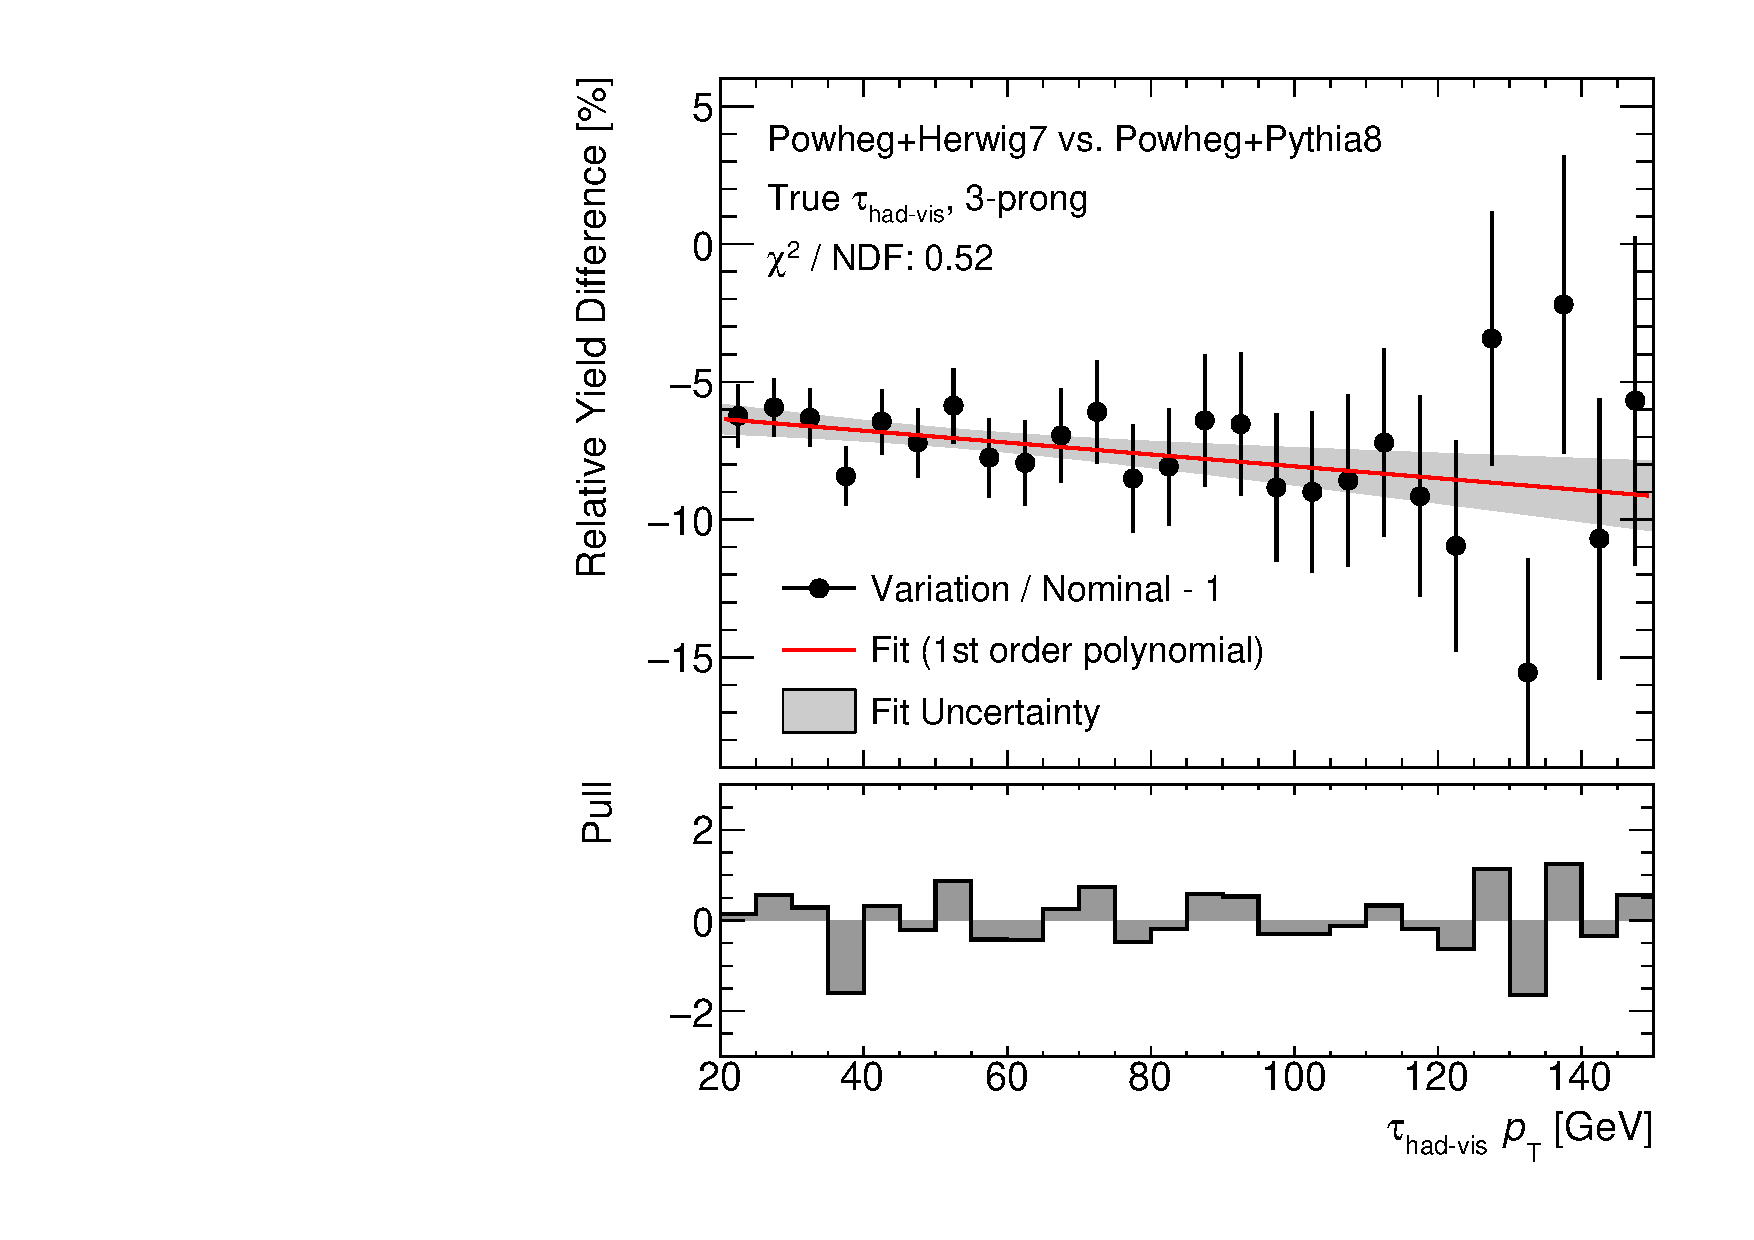
\includegraphics[width=\textwidth]{ttbarSF/uncertainties/ps_true_3p_pt}
    \caption{Impact of the PS variation on \tauhadvis \pT for 3-prong
      \tauhadvis.}
    \label{fig:ttbarSF_uncertainty_ps_3p_pt}
  \end{subfigure}\hfill%
  \begin{subfigure}[t]{.48\textwidth}
    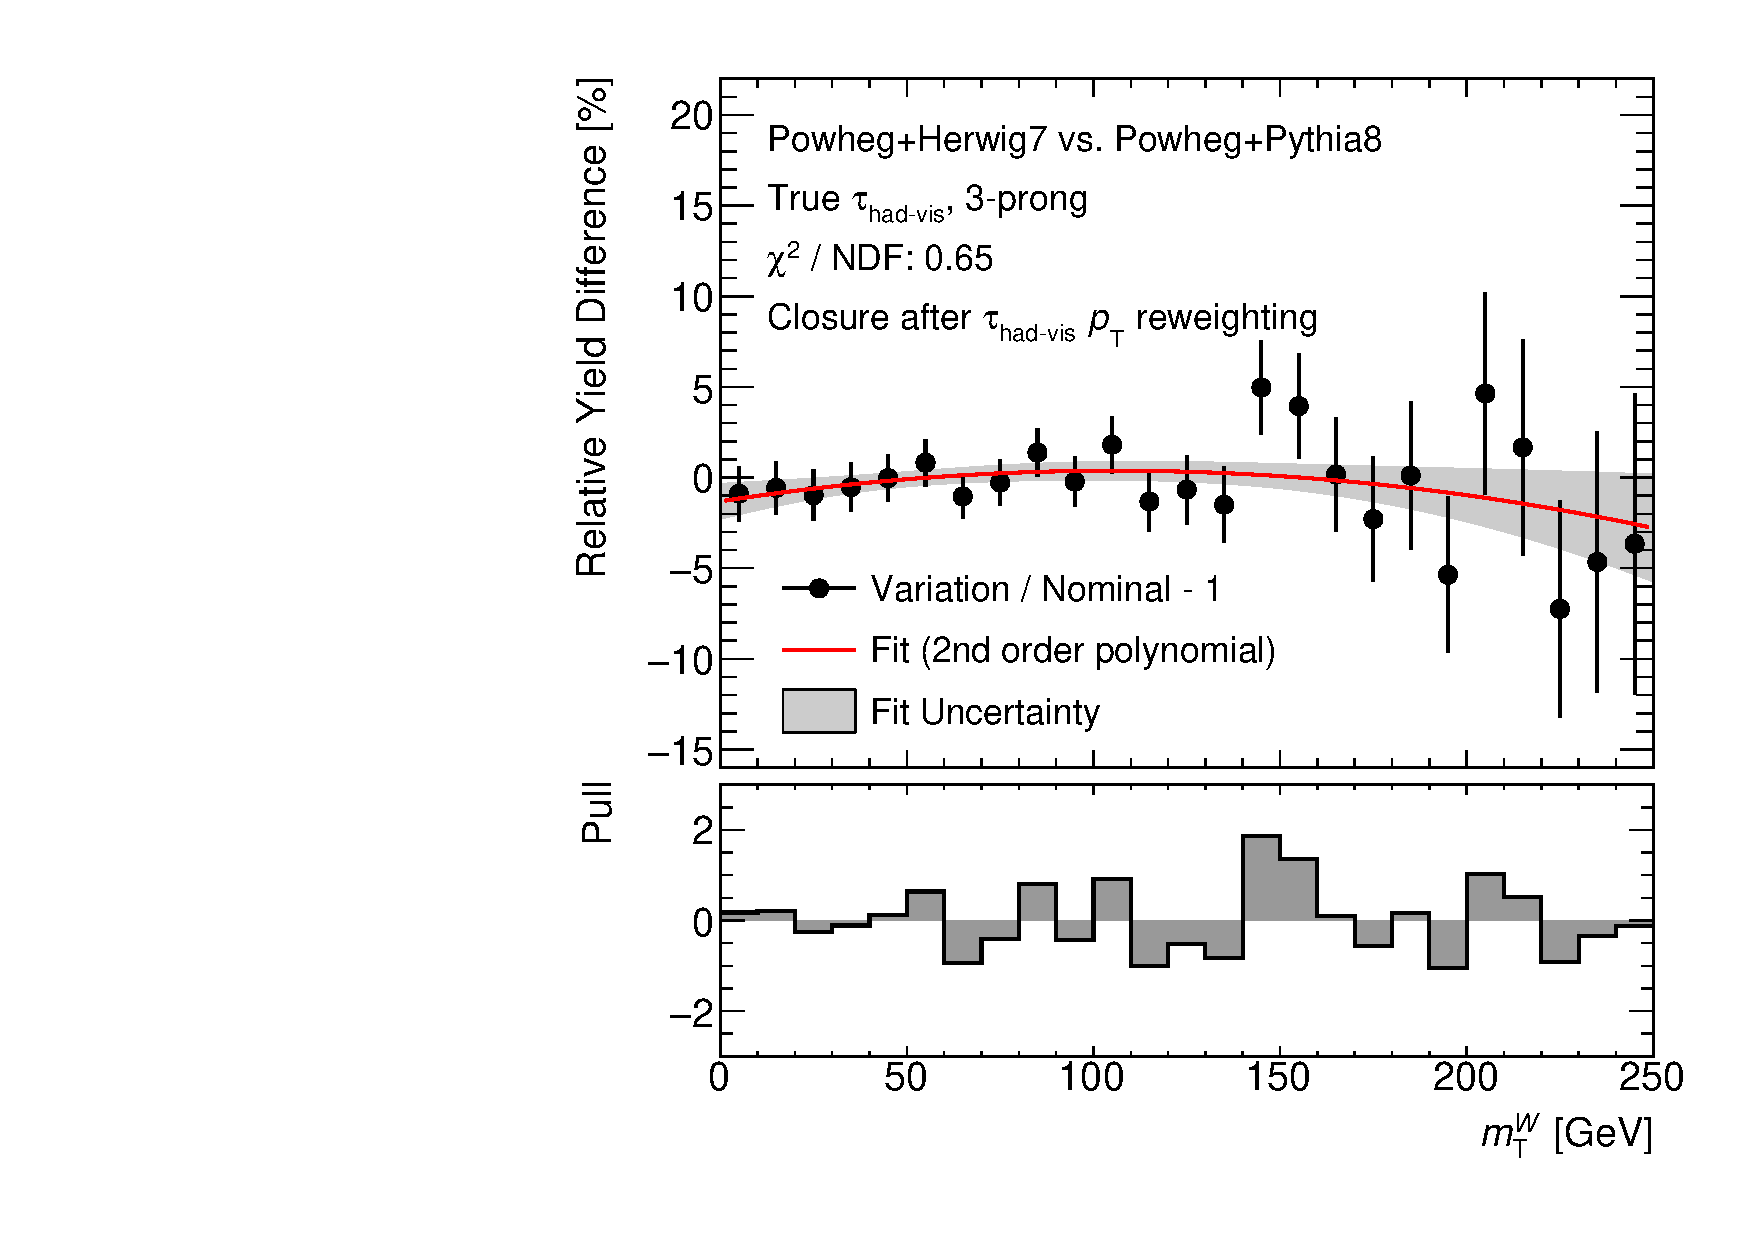
\includegraphics[width=\textwidth]{ttbarSF/uncertainties/ps_true_3p_mtw}
    \caption{Non-closure in \mTW of the PS variation for 3-prong
      \tauhadvis after reweighting the nominal simulation sample.}
    \label{fig:ttbarSF_uncertainty_ps_3p_mtw}
  \end{subfigure}

  \caption{Parton shower and hadronisation model uncertainties from
    the two-sample comparison of the nominal sample (\POWHEGBOX[v2] +
    \PYTHIA[8]) with the variation (\POWHEGBOX[v2] +
    \HERWIG[7]). Shown are the uncertainty for 1-prong (a,b) and
    3-prong (c,d) \tauhadvis matched to true \tauhad. The lower
    threshold on \tauhadvis \pT was relaxed to \SI{20}{\GeV} (from
    \SI{25}{\GeV}) compared to the top control region.}
  \label{fig:ttbarSF_uncertainty_ps}
\end{figure}

\todo{Maybe discuss later that polynomial regression is not so
  well-defined theoretically.}

% The alternative parton shower has the largest effect on the
% modelling of \faketauhadvis.

Acceptance uncertainties on \ttbar with \faketauhadvis are assigned as
shape-only uncertainties in all measurement regions since the
normalisation of this component is extracted in the likelihood fit.
In contrast, the normalisation of \ttbar with true \tauhadvis is not
extracted in each measurement region separately. Therefore, both the
normalisation and the shape effect of the \ttbar acceptance
uncertainties are propagated to the fit for the true \tauhadvis
contribution.

A reduced set of the minor background contributions is considered. For
the production of single top-quarks the uncertainties on the cross
section are applied in the fit. Due to the known normalisation
discrepancy in \Vjets in the presence of jets originating from heavy
flavour, an uncertainty of \SI{30}{\percent} is applied to the overall
normalisation of the process.

The effect of uncertainties on the predicted rates are parametrised by
nuisance parameters that enter the maximum likelihood fit with
Gaussian constraint terms. Uncertainties arising from the same source
are assumed to be fully correlated across all regions and bins.

\todo[inline]{Additional uncertainties are discussed later?}


\subsubsection{Measurement results}

The measured corrections for \faketauhadvis in \ttbar simulation using
\POWHEGBOX[v2]~+~\PYTHIA[8] are shown in
\Cref{fig:ttbarSF_postfit_SF}. The measurement shows varying agreement
between the nominal prediction in simulation and the data-driven
method depending on \tauhadvis~\pT and identification criteria applied
to \tauhadvis candidates. The size of the extracted correction can
reach up to \SI{50}{\percent} at high \tauhadvis \pT where the
simulation overestimates the contribution of \faketauhadvis in \ttbar.

\begin{figure}[htbp]
  \centering

  \begin{subfigure}[t]{.495\textwidth}
    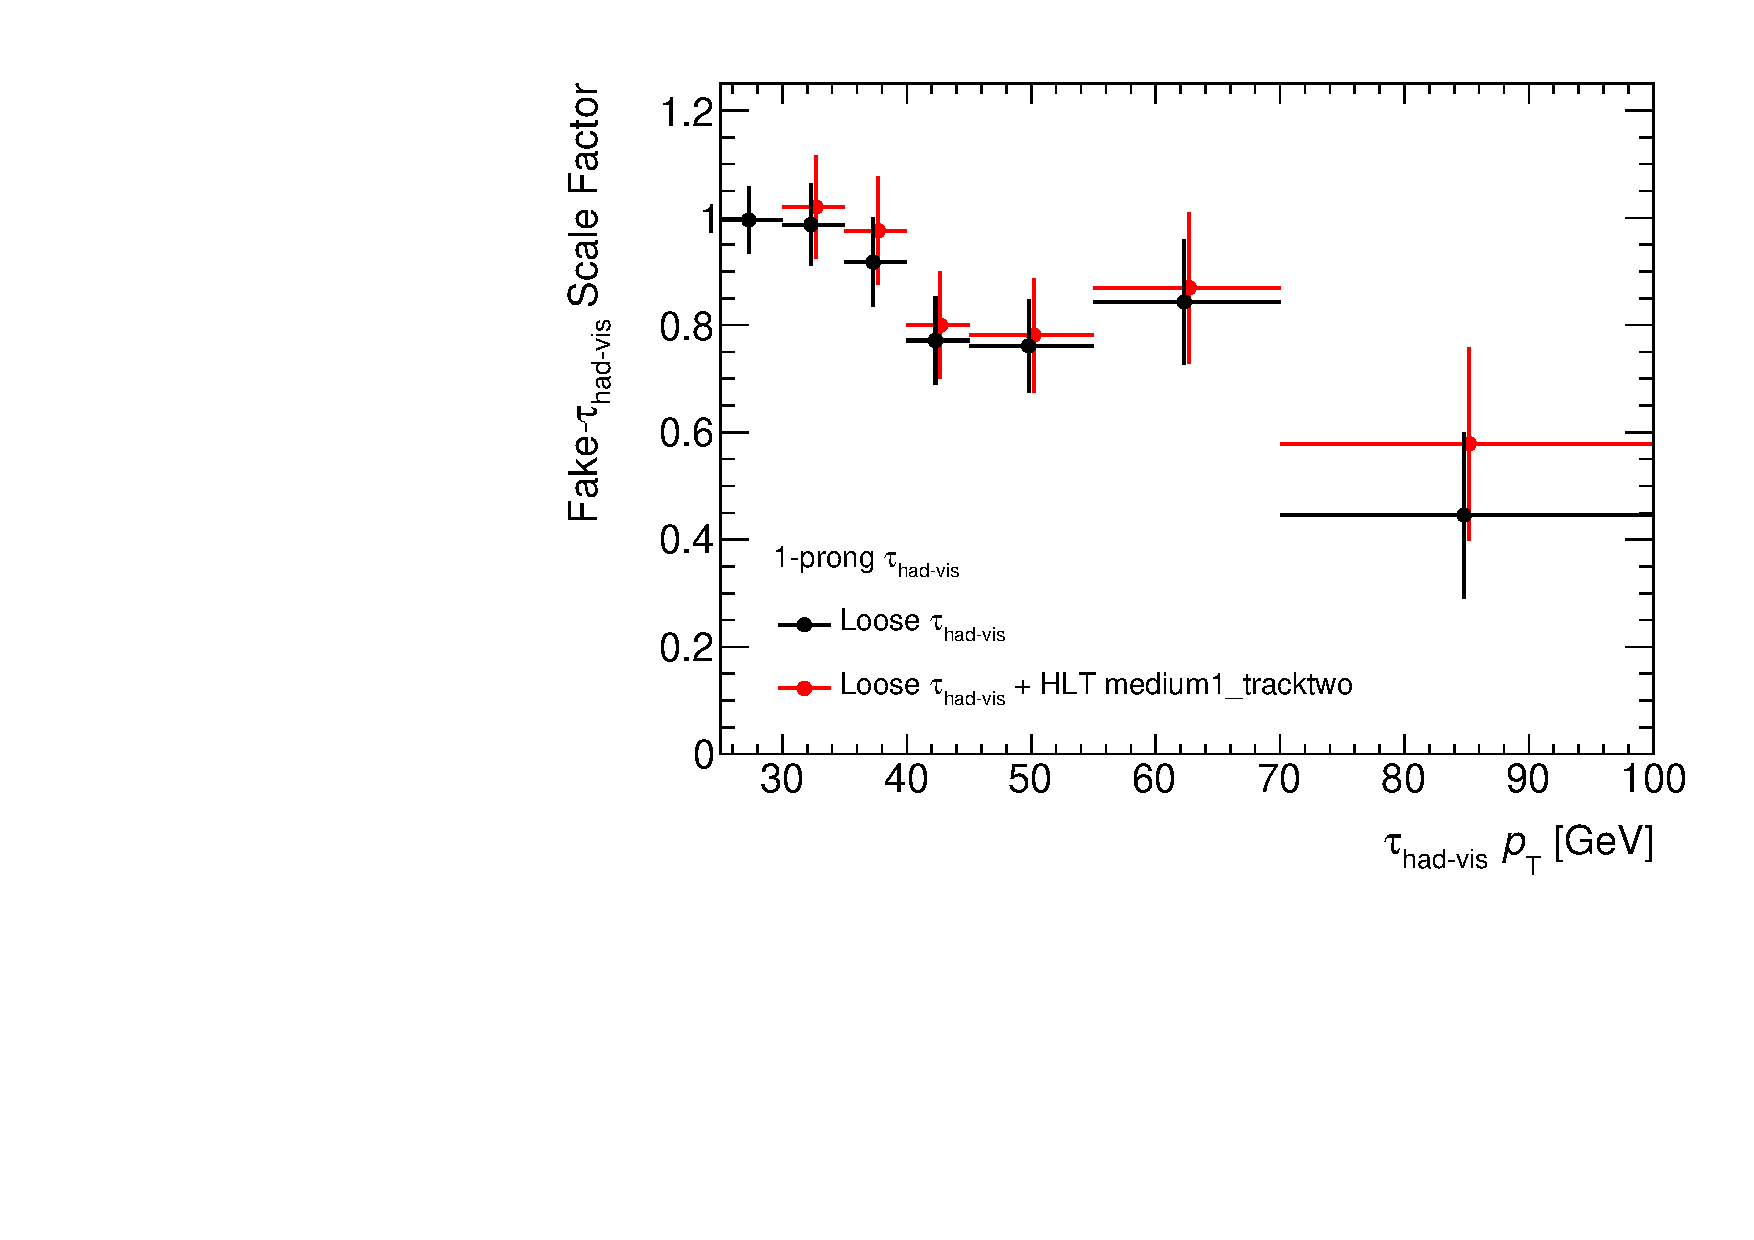
\includegraphics[width=\textwidth]{ttbarSF/ttbarSF_offl_tau25_1p}
    \caption{}
    \label{fig:ttbarSF_postfit_SF_a}
  \end{subfigure}\hfill%
  \begin{subfigure}[t]{.495\textwidth}
    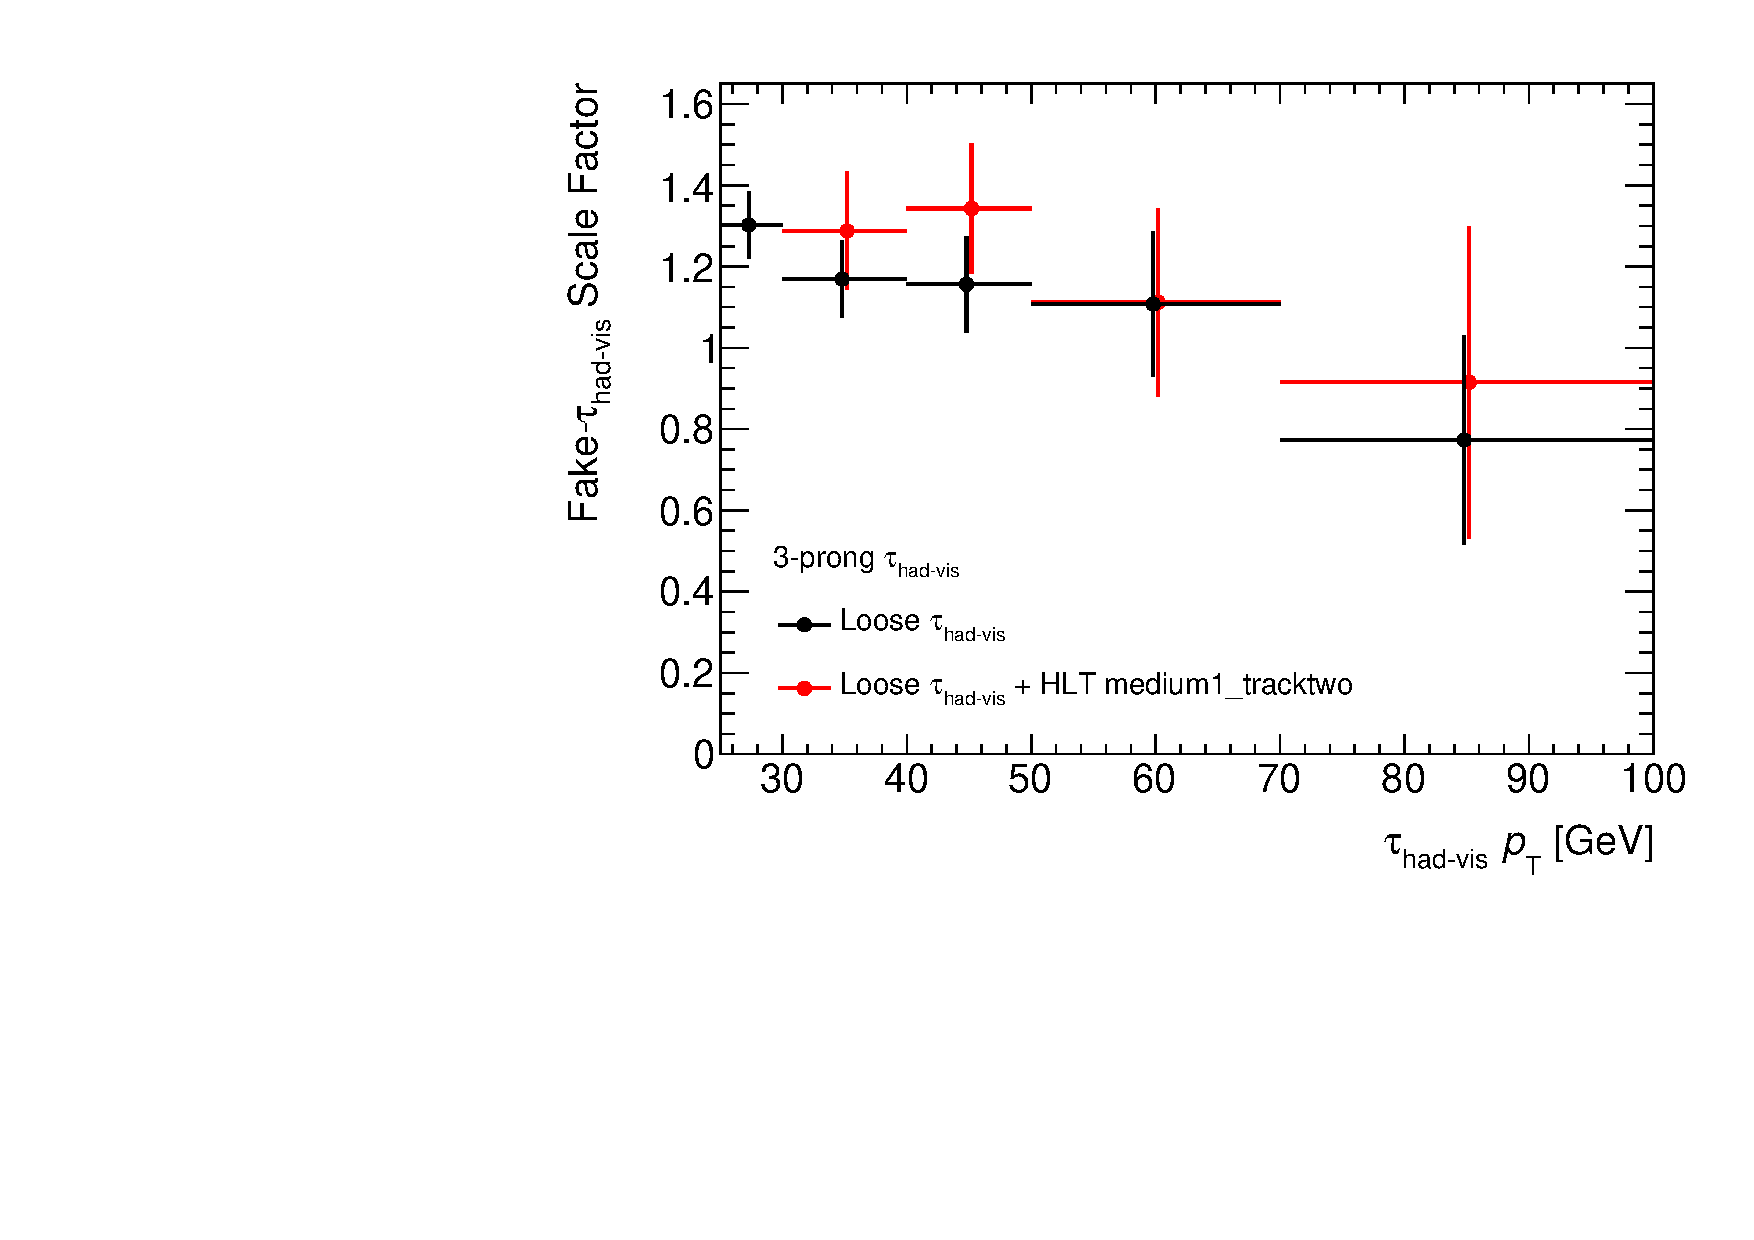
\includegraphics[width=\textwidth]{ttbarSF/ttbarSF_offl_tau25_3p}
    \caption{}
    \label{fig:ttbarSF_postfit_SF_b}
  \end{subfigure}

  \begin{subfigure}[t]{.495\textwidth}
    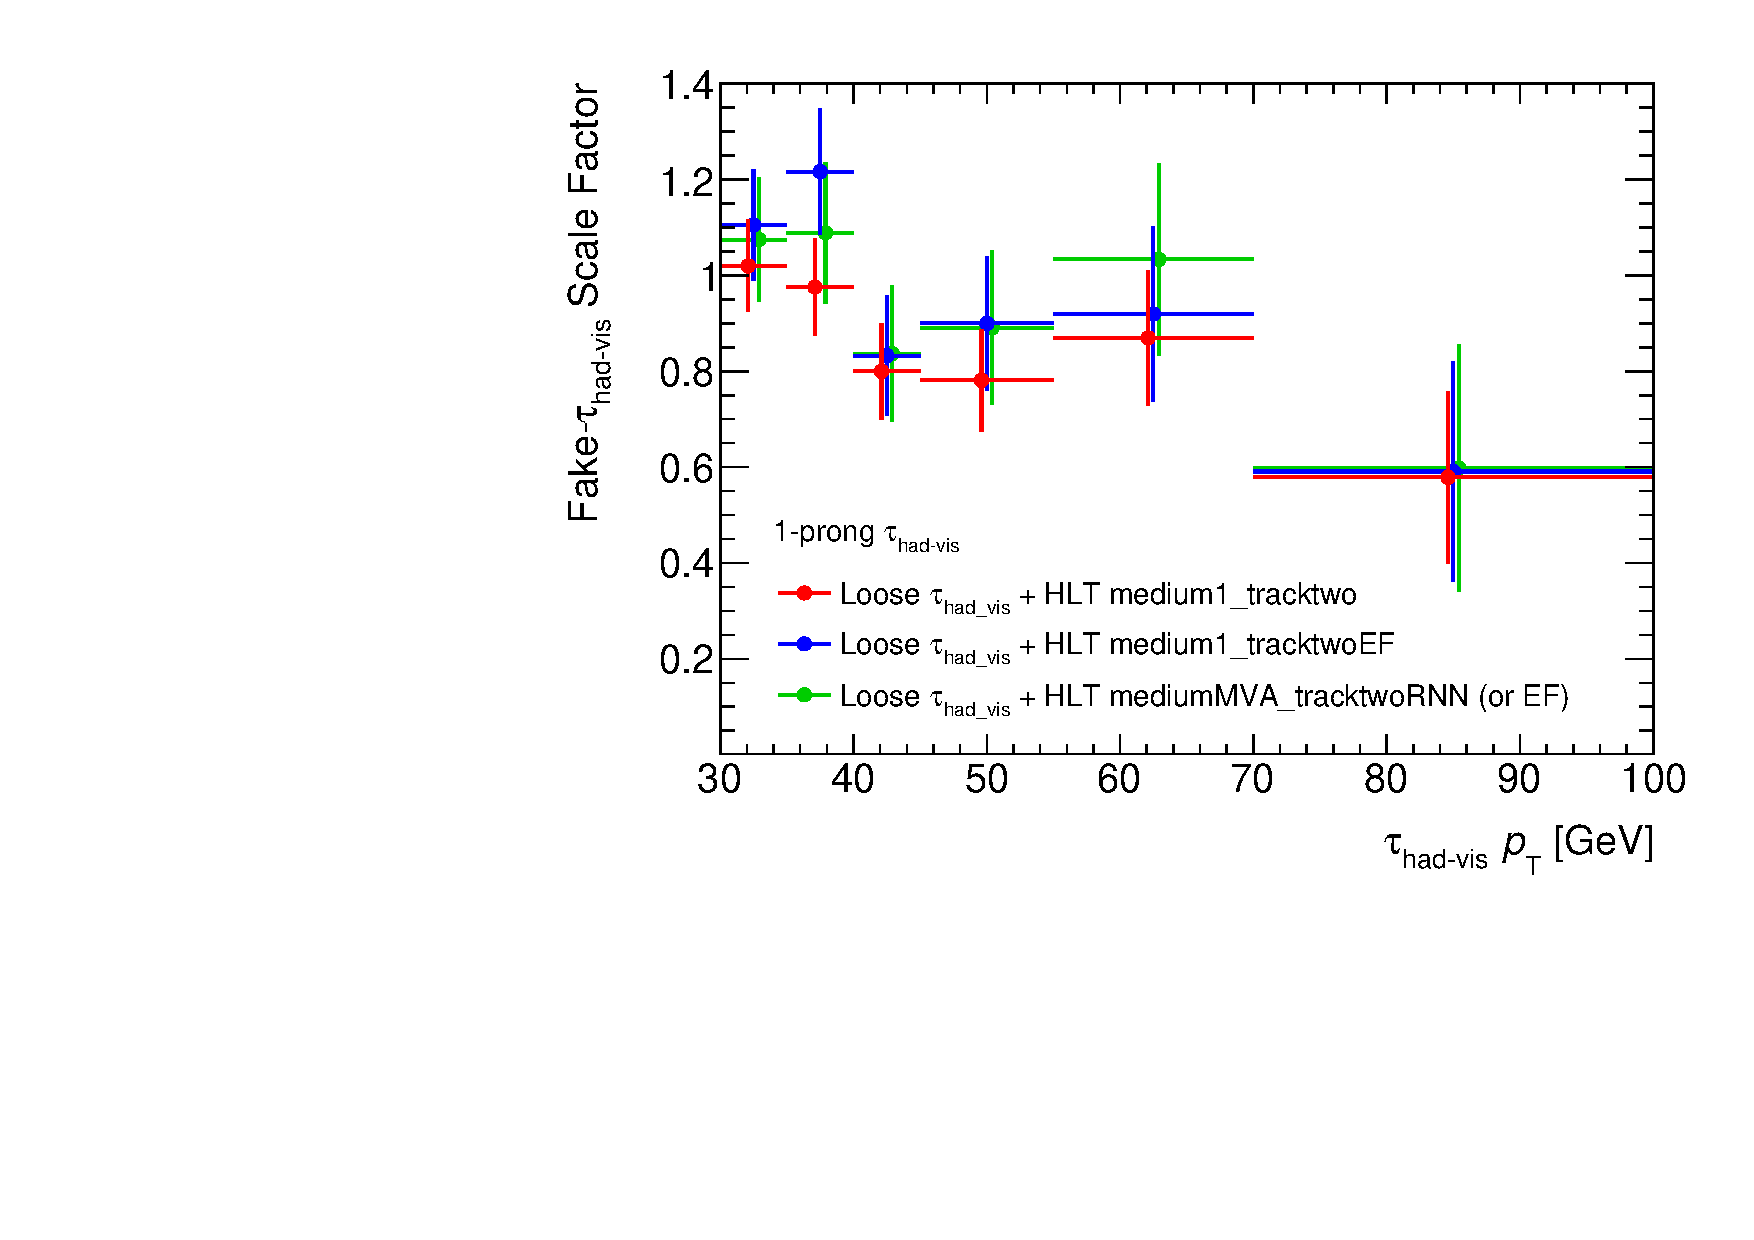
\includegraphics[width=\textwidth]{ttbarSF/ttbarSF_tau25_1p}
    \caption{}
    \label{fig:ttbarSF_postfit_SF_c}
  \end{subfigure}\hfill%
  \begin{subfigure}[t]{.495\textwidth}
    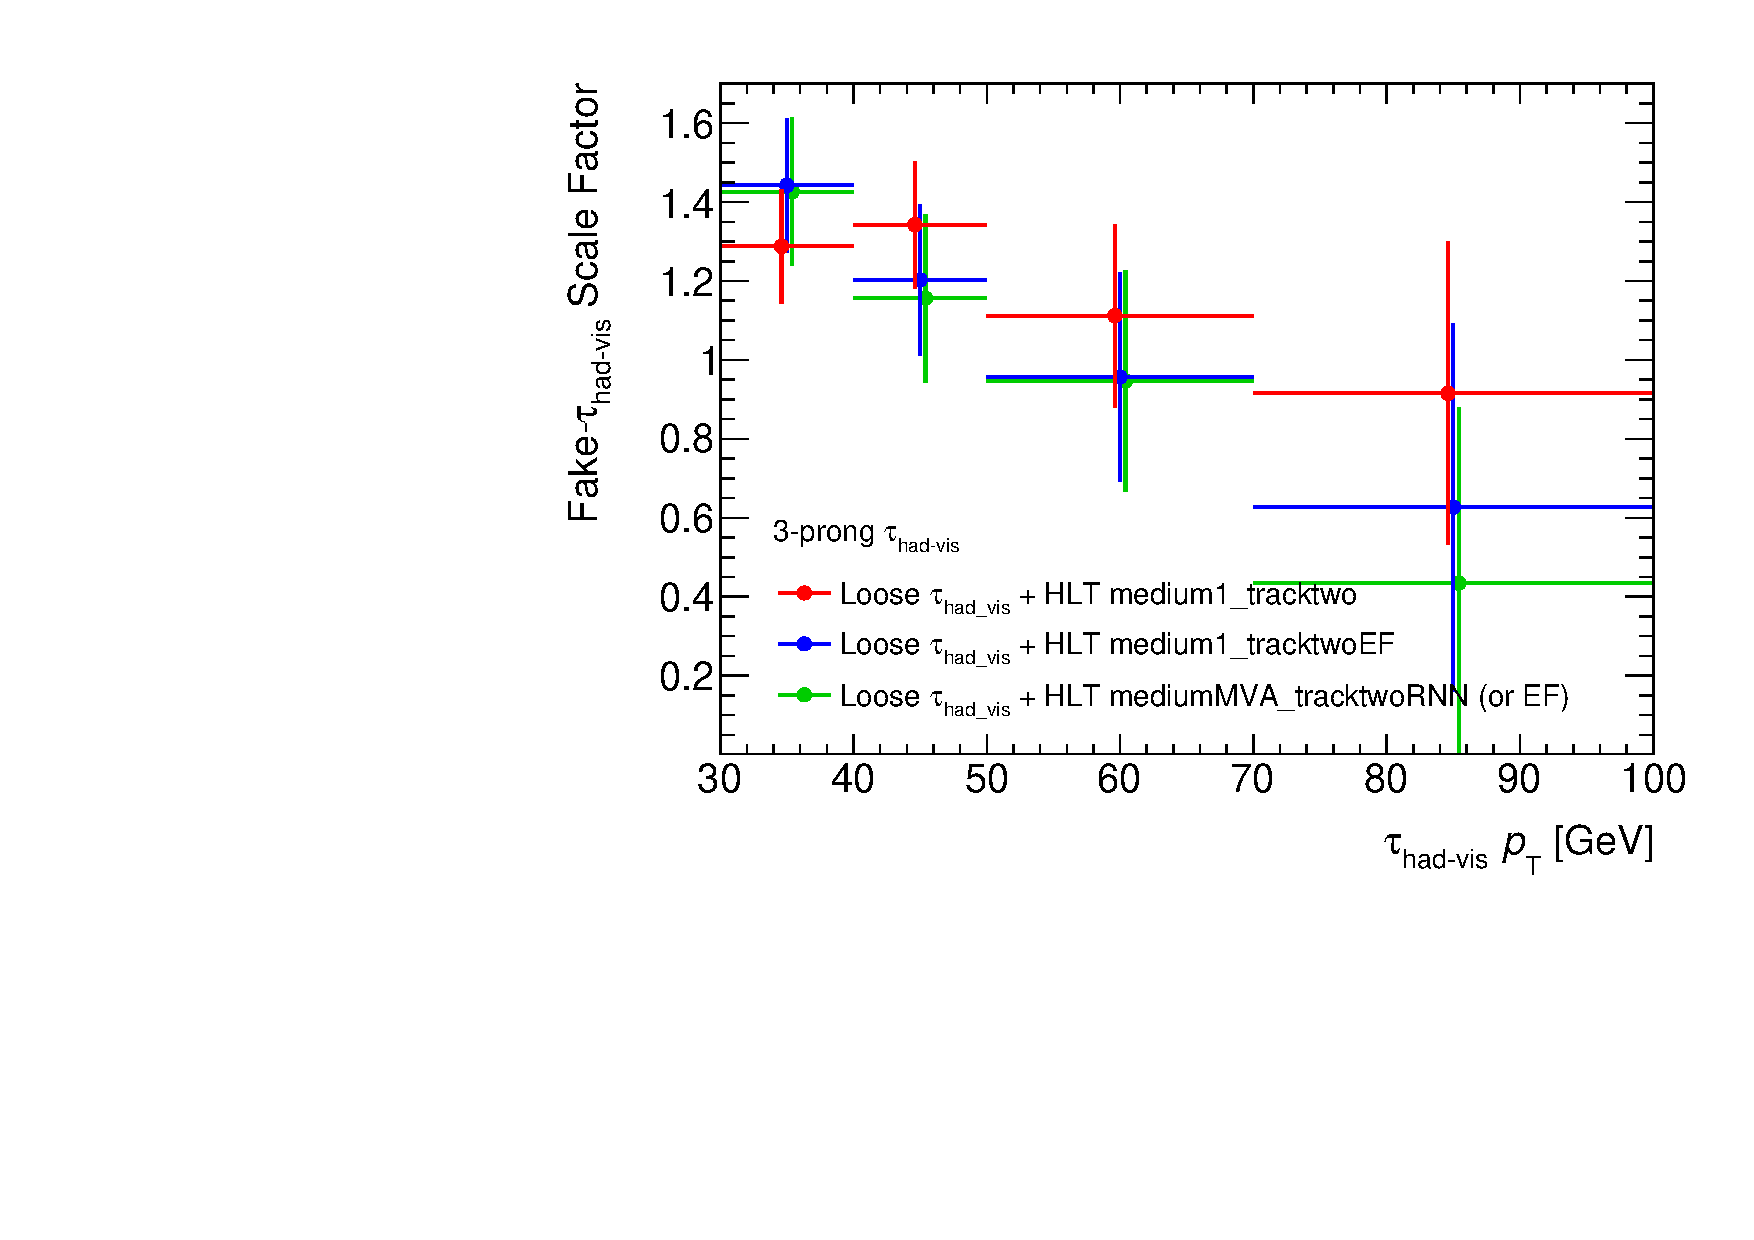
\includegraphics[width=\textwidth]{ttbarSF/ttbarSF_tau25_3p}
    \caption{}
    \label{fig:ttbarSF_postfit_SF_d}
  \end{subfigure}

  \caption{Measured \faketauhadvis scale factors in \ttbar
    (\POWHEGBOX[v2] + \PYTHIA[8]) for all relevant \tauhadvis
    identification criteria used in the analysis. A comparison of
    \faketauhadvis scale factors between loose identification and
    loose~+~HLT~identification is shown in (a) and (b) for 1- and
    3-prong, respecively. Figures (c) and (d) compare the effect of
    different HLT identification algorithms on the extracted scale
    factors. In all cases the last bin summarises events with
    \tauhadvis~$\pT \geq \SI{70}{\GeV}$.  The markers are shifted from
    the geometrical bin center for illustration purposes.}
  \label{fig:ttbarSF_postfit_SF}
\end{figure}

For \faketauhadvis reconstructed as 1-prong \tauhadvis candidates,
depicted in~\Cref{fig:ttbarSF_postfit_SF_a,fig:ttbarSF_postfit_SF_c},
the corrections are of the order of \SI{20}{\percent} in the low and
intermediate transverse momentum regime ($\pTvis < \SI{70}{\GeV}$).
The dependency of the extracted scale factors shows no strong
systematic dependence regarding the \tauhadvis identification applied
at the HLT, and differences in identification algorithms.

In~\Cref{fig:ttbarSF_postfit_SF_b,fig:ttbarSF_postfit_SF_d} the
measured scale factors for \faketauhadvis reconstructed as 3-prong
candidates are shown. For 3-prong candidates the abundance of
\faketauhadvis is underestimated in simulation in the low and
intermediate \tauhadvis~\pT region requiring corrections of
approximately \num{20} to \SI{30}{\percent}. The contribution of
\faketauhadvis in simulation at high momenta tends to be overestimated
although with large measurement uncertainties due to the small
expected contribution of \faketauhadvis. This is further magnified for
the \texttt{medium1\_tracktwoEF} and \texttt{mediumMVA\_tracktwoRNN}
trigger chains where only partial datasets are available for the
measurements.

\todo[inline]{Fit cross checks: pulls, constraints, ranking?}

\todo[inline]{This measurement can provide a correction as well as a
  measurement-driven estimate of the uncertainties of
  \faketauhadvis. Although the uncertainties seem large at high
  momenta, the abundance of events where this is relevant is small.}

The fit model introduces large anti-correlations between the global
\ttbar normalisation and the extracted scale factors for \ttbar with
\faketauhadvis. An exemplary correlation matrix for one measurement is
shown in~\Cref{fig:ttbarSF_corr_matrix} showing the most relevant
correlations between parameters of interest and nuisance parameters.
The anti-correlations are a result of the limited discrimination power
of \mTW in distinguishing between \ttbar with true- and \faketauhadvis
which is especially poor for low \tauhadvis transverse momenta. Thus a
change in the global \ttbar normalisation, affecting both \ttbar with
true and \faketauhadvis, can be partially compensated by an increase
in the \faketauhadvis scale factors. This coupling between scale
factors and global \ttbar normalisation introduces large positive
correlations also between the scale factors themselves.

\begin{figure}[htbp]
  \centering
  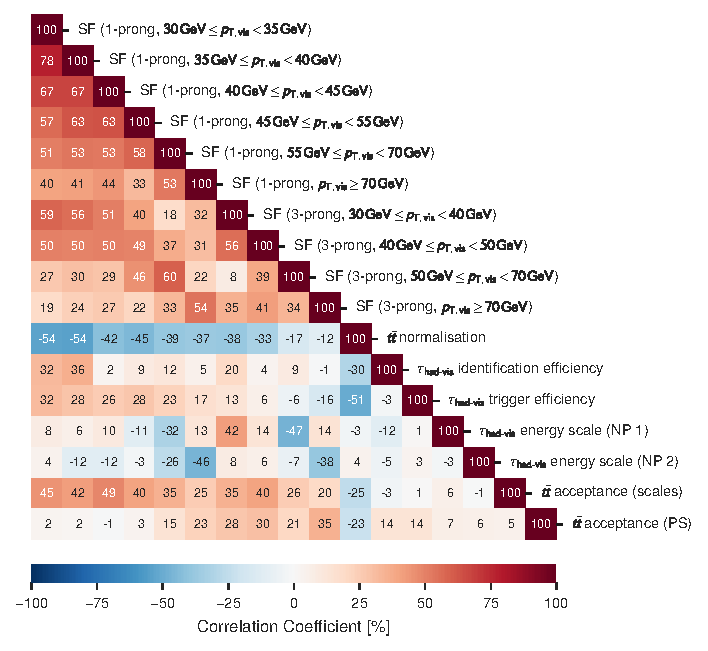
\includegraphics[scale=0.88]{ttbarSF/correlation_matrix}

  \caption{Correlation matrix at the maximum likelihood estimate of
    the fit model for the scale factor measurement of the
    \texttt{HLT\_tau25\_medium1\_tracktwo} trigger. A reduced number
    of parameters is shown for illustration purposes. Nuisance
    parameters are included if the absolute value of its correlation
    coefficient exceeds \SI{30}{\percent} with at least one parameter
    of interest.}
  \label{fig:ttbarSF_corr_matrix}
\end{figure}

Correlations between the extracted scale factors needs to be taken
into account when propagating the measurement uncertainties to the
estimate of \ttbar with \faketauhadvis in the \hadhad signal region. A
convenient method to achieve this is by providing decorrelated
variations of the measurement that jointly explain the total
uncertainty of all scale factors. These sets of scale factor
variations can be used to propagate the uncertainties without having
to account for correlations.

A decorrelated set of variations can be obtained by a linear
transformation procedure of the $N$~original scale factors. The
necessary transformation is obtained by diagonalising the post-fit
covariance matrix resulting in a set of eigenvectors and
eigenvalues. The eigenvectors provide an alternative basis in which
the measurement is described by $N$~linear combinations of SFs. The
covariance between two different linear combinations is zero by
construction and the eigenvalues describe the variance of individual
linear combinations. This decomposition is used to construct
decorrelated variations of the SF measurement by performing
$\pm 1 \sigma$ variations in the frame with diagonal covariance
matrix, followed by a transformation to the original frame (with
non-diagonal covariance matrix). This procedure yields $N$ variations
of the scale factor measurement each with an up- and
down-variation\footnote{The notion of up- and down-variations is
  merely mathematical, i.e.\ according to the variation in the
  diagonal frame, and does not have a concrete physical meaning.}. The
variations are ordered in descending variance in the diagonal frame
and thus the effect size of the variation on the background estimate
is also expected to approximately follow a descending order\todo{Maybe
  clarify why it is only approximate.}. An example of this
decomposition is shown in~\Cref{fig:ttbarSF_eigenvariations}. The
effect of large correlations between scale factors can be seen in the
leading variation (\texttt{EIGEN0}) as a systematic shift of the SF
variation in the same direction with respect to the nominal scale
factors.

\begin{figure}[htbp]
  \centering

  \begin{subfigure}[t]{.495\textwidth}
    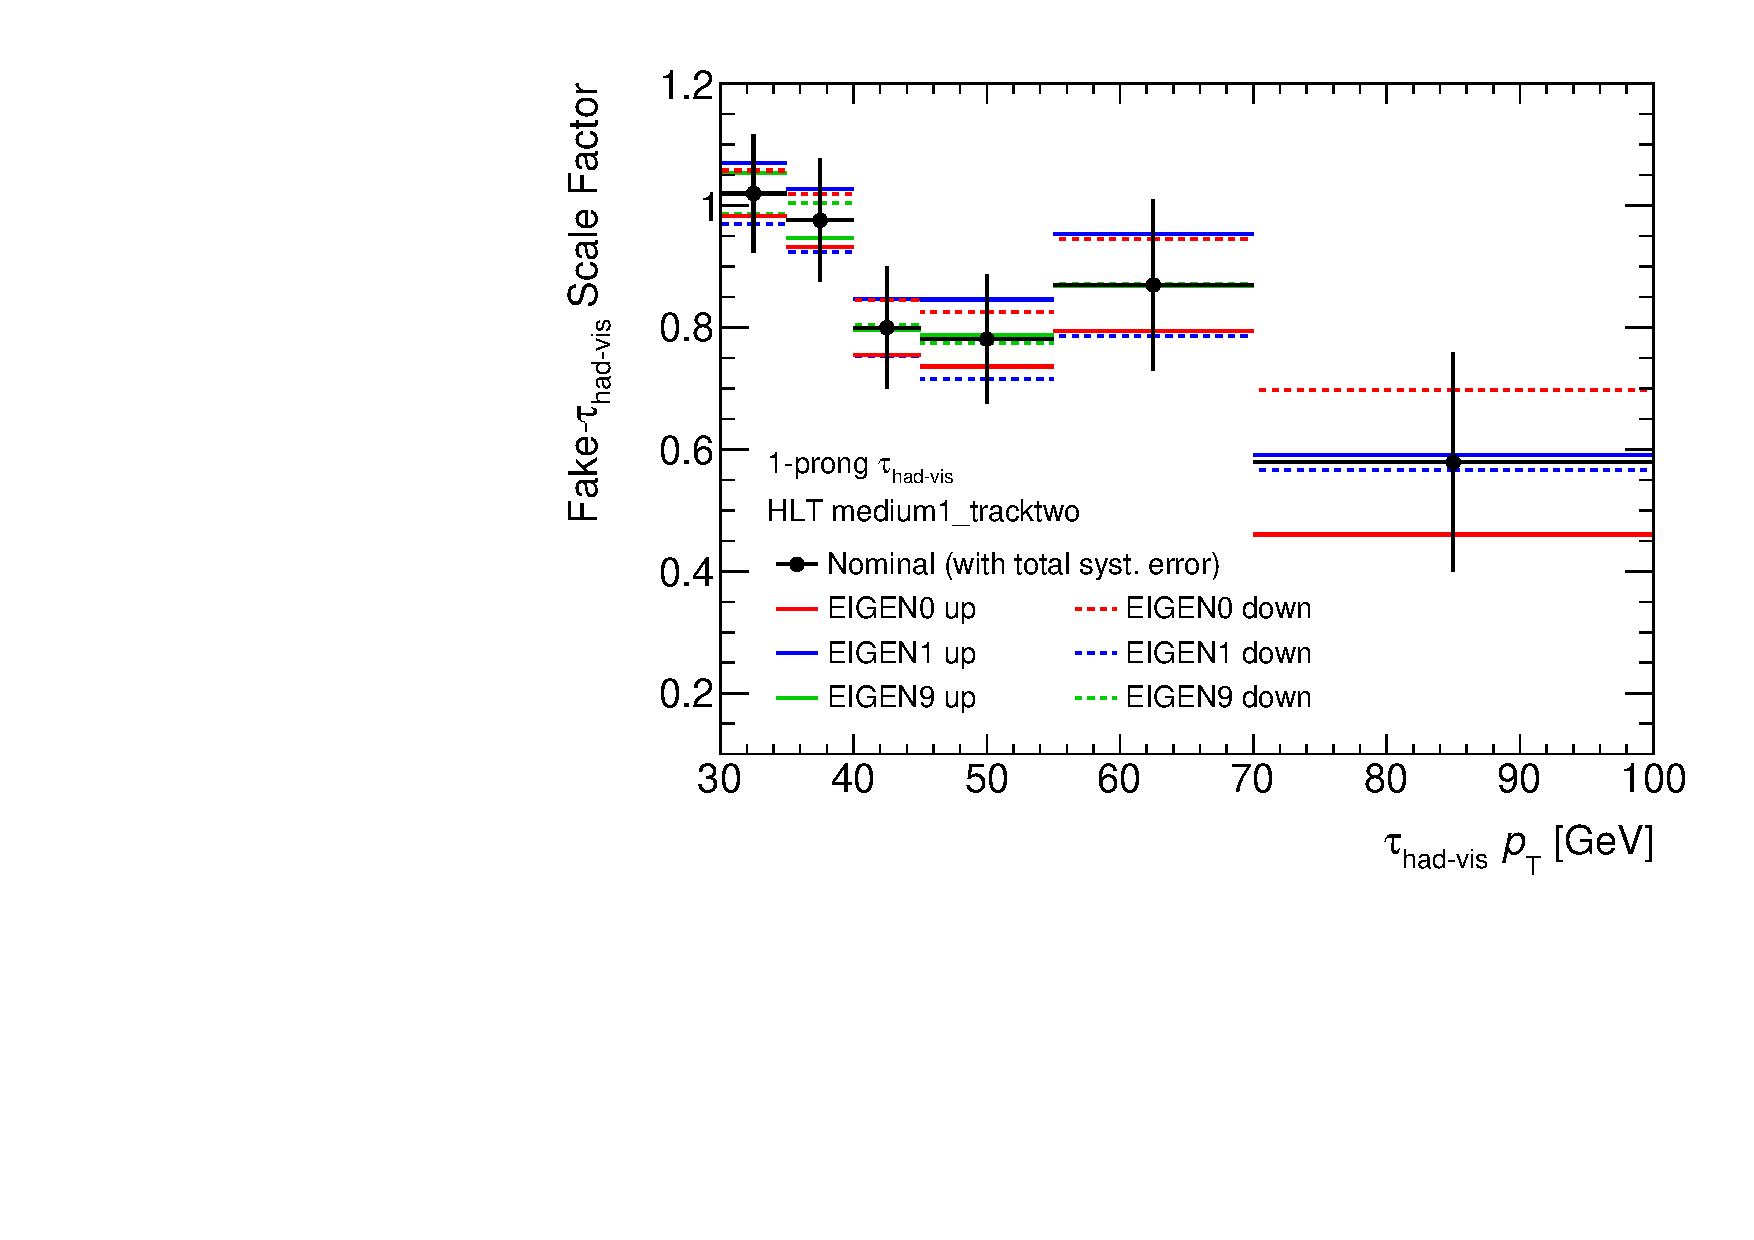
\includegraphics[width=\textwidth]{ttbarSF/ttbarSF_eigvar_1p}
    \caption{1-prong \tauhadvis}
    \label{fig:ttbarSF_eigenvariations_1p}
  \end{subfigure}\hfill%
  \begin{subfigure}[t]{.495\textwidth}
    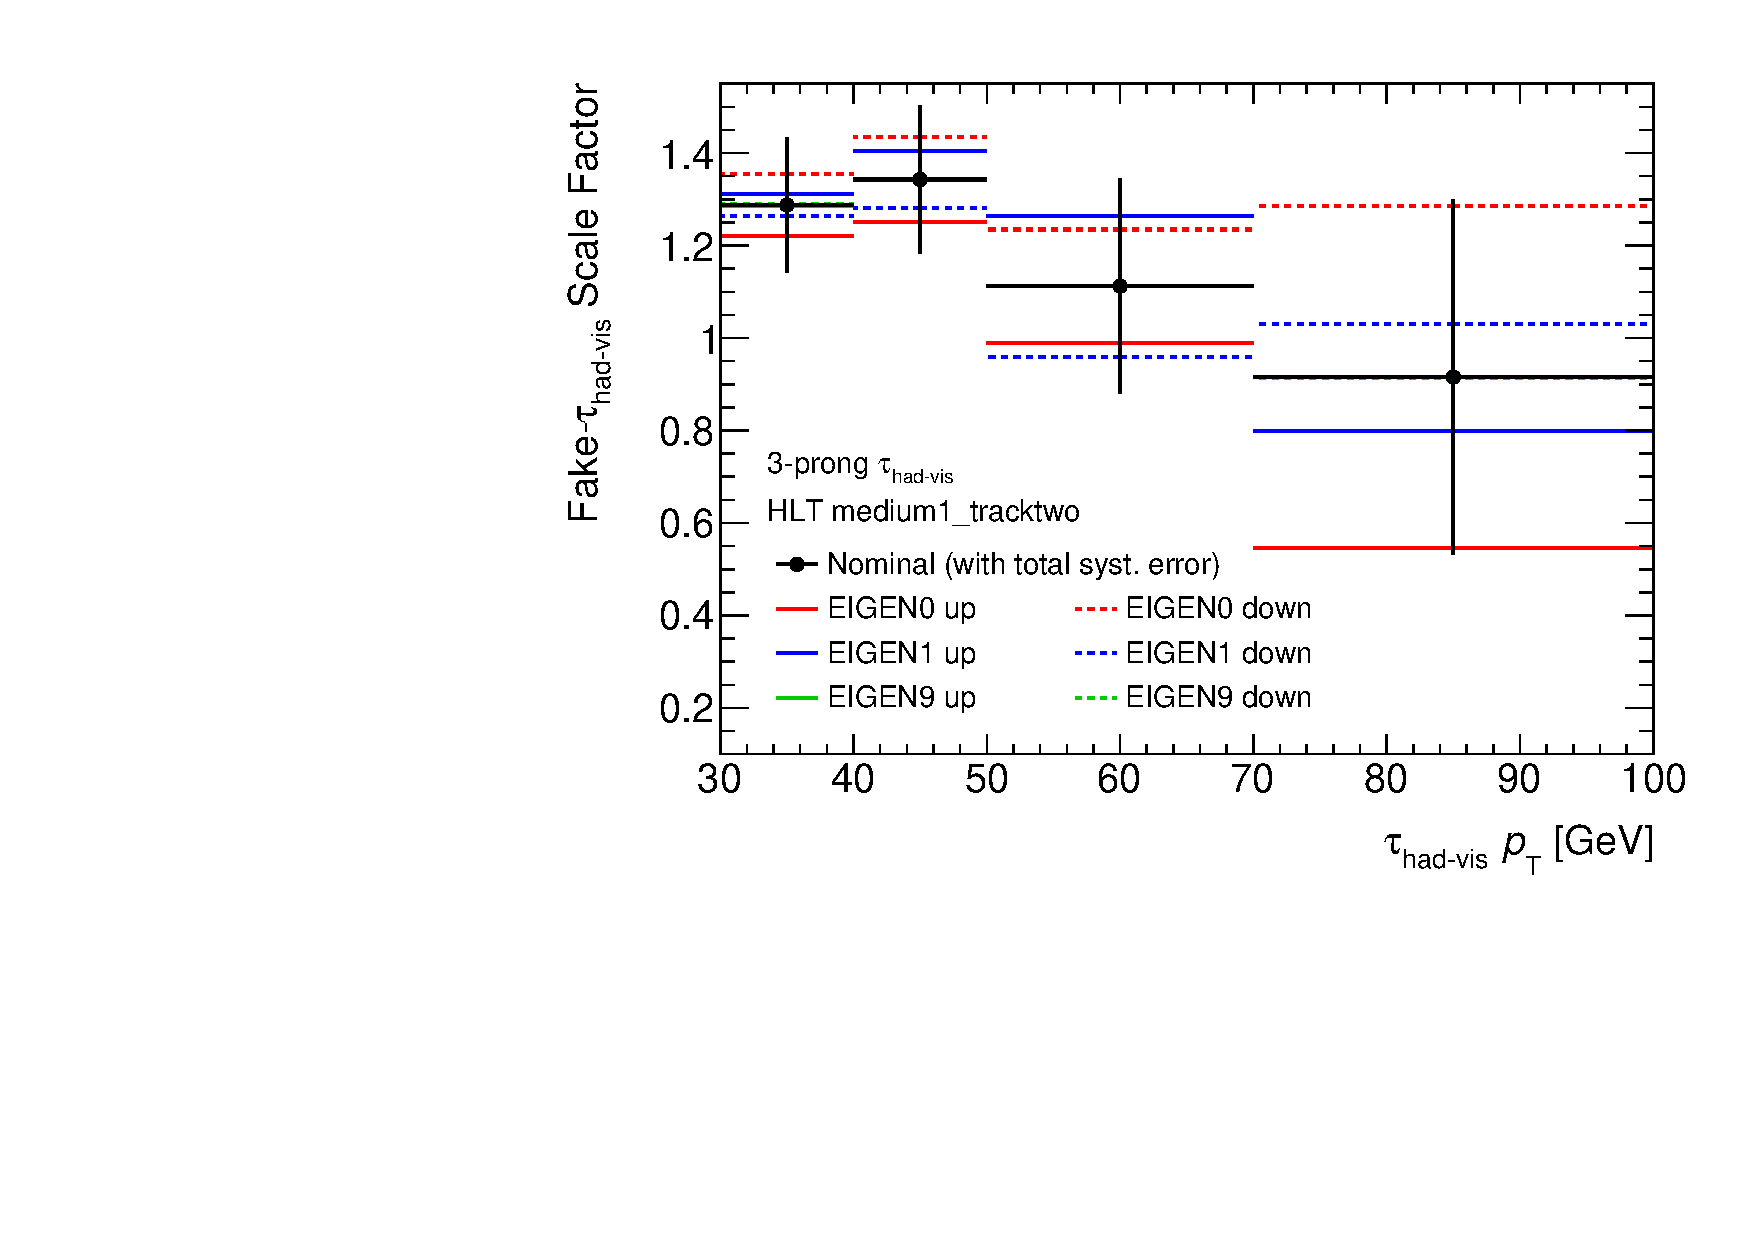
\includegraphics[width=\textwidth]{ttbarSF/ttbarSF_eigvar_3p}
    \caption{3-prong \tauhadvis}
    \label{fig:ttbarSF_eigenvariations_3p}
  \end{subfigure}

  \caption{Variations resulting from the decorrelation procedure for
    the scale factor measurement of \tauhadvis passing matching to the
    \texttt{HLT\_tau25\_medium1\_tracktwo} trigger. Shown are the two
    variations explaining most of the variance, \texttt{EIGEN0} and
    \texttt{EIGEN1}, and the variation explaining the least variance,
    \texttt{EIGEN9}. Adding the deviations of all SF variations
    (\texttt{EIGEN0} - \texttt{EIGEN9}) from the nominal result in
    quadrature recovers the total systematic error.}
  \label{fig:ttbarSF_eigenvariations}
\end{figure}


\subsubsection{Application}

An estimate of the \ttbar background with \faketauhadvis in the SR of
the \hadhad channel can be obtained by applying suitable scale factors
to events containing at least one \faketauhadvis in \ttbar simulation.
These events are required to pass the signal region selection criteria
of the \hadhad channel. This includes the event being selected by a
trigger according to the selection strategy outlined
in~\Cref{sec:trigger} and the reconstructed \tauhadvis candidates
being matched to \tauhadvis at the HLT accordingly.

The scale factors are chosen depending on the trigger category and
whether the \faketauhadvis is the \tauhadvis candidate leading in \pT,
subleading in \pT, or whether both candidates are originating from
quark- or gluon-jets. In cases where both \tauhadvis faked by jets,
the correction is assumed to factorise and the product of scale
factors is assigned as the event weight.

In events selected by di-\tauhadvis triggers both \tauhadvis
candidates have to pass identification requirements at the HLT. In
this case the scale factor measurement is chosen according to the
active trigger chain, independent on which \tauhadvis candidate is
originating from a jet. In events selected by single-\tauhadvis
triggers at leaast one \tauhadvis candidate is required to pass the
HLT \tauhadvis identification requirement. A simplification is made
assuming that the \tauhadvis candidate leading in \pT passed the HLT
\tauhadvis identification, causing the event to be selected by the
trigger. This assumption is valid for more than \SI{99}{\percent} of
\ttbar events containing \faketauhadvis in the STT
category. Therefore, scale factors with HLT identification are applied
when the leading \tauhadvis is faked by a jet; scale factors without
HLT identification are applied when the subleading \tauhadvis is faked
by a jet. Similar to the di-\tauhadvis trigger case, the set of scale
factors for the candidate passing HLT identification is chosen
according to the active trigger chain. The event weight calculation is
summarised in~\Cref{tab:ttbarSF_application_rule}.

\begin{table}[htbp]
  \centering

  \begin{tabular}{cc@{\hskip 2em}rcl@{\hskip 2em}rcl}
  \toprule
  $\tau_{\text{lead.}}$ & $\tau_{\text{subl.}}$ & \multicolumn{3}{c}{Event weight (STT)} & \multicolumn{3}{c}{Event weight (DTT)} \\
  \midrule
  true & fake & $1$ & $\times$ & $\text{SF}_\text{loose}(\tau_{\text{subl.}})$
              & $1$ & $\times$ & $\text{SF}_\text{loose+trig.}(\tau_{\text{subl.}})$ \\[0.2em]

  fake & true & $\text{SF}_\text{loose+trig.}(\tau_{\text{lead.}})$ & $\times$ & $1$
              & $\text{SF}_\text{loose+trig.}(\tau_{\text{lead.}})$ & $\times$ & $1$ \\[0.2em]

  fake & fake & $\text{SF}_\text{loose+trig.}(\tau_{\text{lead.}})$ & $\times$ & $\text{SF}_\text{loose}(\tau_{\text{subl.}})$
              & $\text{SF}_\text{loose+trig.}(\tau_{\text{lead.}})$ & $\times$ & $\text{SF}_\text{loose+trig.}(\tau_{\text{subl.}})$ \\
  \bottomrule
\end{tabular}

%%% Local Variables:
%%% mode: latex
%%% TeX-master: "../phd_thesis"
%%% End:


  \caption{Construction of the multiplicative event weight for
    data-driven correction of \ttbar with \faketauhadvis in
    simulation. Events are distinguished whether the leading
    \tauhadvis candidate ($\tau_{\text{lead.}}$), the subleading
    \tauhadvis candidate ($\tau_{\text{subl.}}$), or both are faked by
    a jet.  Scale factors for \faketauhadvis without HLT trigger
    identification, i.e.\ only with loose offline \tauhadvis
    identification, are denoted as $\text{SF}_{\text{loose}}$;
    scale factors with HLT trigger identification as
    $\text{SF}_\text{HLT}$. The set of scale factors after HLT
    \tauhadvis identification is chosen according to the trigger
    algorithm used during the run where the event occurred.}
  \label{tab:ttbarSF_application_rule}
\end{table}

% When applying the scale factors to events in the 𝜏 had 𝜏 had -channel,
% an approach similar to the application of true 𝜏 had calibrations
% (e.g. trigger and offline 𝜏 had ), where it is assumed that the
% calibrations factorize in a multi-𝜏 had final state, is taken. In this
% analysis this assumption only affects the 𝑡 𝑡 ¯ final state with two
% fake 𝜏 had (FF events). This contribution is a subleading source of
% fake 𝜏 had making up only 15 % of the
% total 𝑡 𝑡 ¯ +fake 𝜏 had contribution (the dominant contributions are
% events where only one 𝜏 had is fake – i.e.  TF and FT events). The
% uncertainties related to the fake scale factor measurement are assumed
% to be
% fully correlated between both 𝜏 had in DTT FF events 12 and are
% propagated as such to the final background estimate in the 𝜏 had 𝜏 had
% -channel. Compared to the size of the uncertainties affecting FF
% events (e.g. 40 %
% for the 𝜏 lep 𝜏 had → 𝜏 had 𝜏 had extrapolation uncertainties,
% c.f. Table 24), deviations from this assumption are thought to be
% negligible.


\begin{table}[htbp]
  \centering

  % Source:
% https://docs.google.com/spreadsheets/d/1uwVElPaR1HuqEHaL8eAh5pEoGdK2ZBQ8D_Ob8lSSPwE/edit#gid=0

% fSumw[1]=2705.09, x=0.5, error=22.9788

% Only measurement uncertainties
% ttbarSFTF: 1433.95 +- 87.88
% ttbarSFFT: 698.52 +- 72.21
% ttbarSFFF: 358.92 +- 53.50
% Total: 2491.39 +- 21.59 +- 202.99 = 204.13493

\begin{tabular}{
  l
  @{\hskip 16pt}
  S[table-format=4.0(2)]
  @{\hskip 16pt}
  S[table-format=4.0(3)]
  }
  \toprule
  & \multicolumn{2}{c}{Expected number of events (pre-fit)} \\
  \cmidrule{2-3}
          & {Simulation} & {Simulation with} \\
  Process &              & {\faketauhadvisC SF}  \\
  \midrule
  \ttbar + \faketauhadvisC (TF) & 1428 +- 16 & 1430 +- 230 \\
  \ttbar + \faketauhadvisC (FT) & 854 +- 13 & 699 +- 88 \\
  \ttbar + \faketauhadvisC (FF) & 423 +- 12 & 360 +- 160 \\
  \midrule
  \ttbar + \faketauhadvisC (total) & 2705 +- 23 & 2490 +- 320 \\
  \bottomrule
\end{tabular}

%%% Local Variables:
%%% mode: latex
%%% TeX-master: "../phd_thesis"
%%% End:


  \caption{Total yield of simulated \ttbar with \faketauhadvis in the
    \hadhad SR before and after correction using the measured scale
    factors. The uncorrected yield is shown with MC statistical
    uncertainties only; the corrected yield with MC statistical, and
    systematic uncertainties of the SF measurement.}
  \todo[inline]{Rather put in all uncertainties?}
  \label{tab:ttbarSF_yields}
\end{table}

\todo[inline]{More comparison of fake estimates?}

\todo[inline]{There need to be some validation checks here...}


\subsubsection{Systematic uncertainties}

\todo[inline]{How does STT play into this? The momentum thresholds are
  unrealistically high so that it can barely be measured with this
  approach.}

A systematic uncertainty measuring the effect of different transverse
momentum thresholds on \tauhadvis at the HLT is derived.  Events
selected by di-\tauhadvis triggers have \tauhadvis exceeding
\pTHLT~thresholds of \SI{35}{\GeV} and \SI{25}{\GeV} for the leading
and subleading candidate, respectively. These triggers only differ in
the \pTHLT~threshold with isolation and identification requirements
remaining the same.

The estimate of the \ttbarFakes background where the \faketauhadvis is
required to pass trigger-matching employs scale factors measured for
triggers with $\pTHLT > \SI{25}{\GeV}$, primarily targeting the effect
of isolation and identification requirements, thus neglecting
differences due to the \pTHLT~selection. This is an approximation for
cases where the leading \tauhadvis candidate in the DTT category is
mimicked by a jet and is motivated by the large overlap in events
selected by both triggers beyond the $\pTvis > \SI{40}{\GeV}$
threshold applied to the leading \tauhadvis in the DTT category at
offline reconstruction-level.

The overlap is studied in simulated \ttbar with at least one
\faketauhadvis in the top control region by examining the
condiditional probability of an event passing the
$\pTHLT > \SI{35}{\GeV}$~trigger provided the event passes
$\pTHLT > \SI{25}{\GeV}$, depending on \pTvis after offline \tauhadvis
reconstruction. Over the \pTvis threshold of \SI{40}{\GeV}, the
overlap between both triggers is \SI{95}{\percent} for \faketauhadvis
reconstructed as 1-prong candidates; \SI{85}{\percent} for
\faketauhadvis reconstructed as 3-prong candidates\todo{Overlap plot
  from INT? Worse for 3-prong due to poorer energy resolution.}.  With
increasing \pTvis the overlap further increases reaching close to full
overlap for $\pTvis > \SI{50}{\GeV}$ for 1-prong, and
$\pTvis > \SI{60}{\GeV}$ for 3-prong candidates. No uncertainty is
applied beyond this point due to negligible differences between
triggers.

The scale factor measurement is repeated after requiring matching to
single-\tauhadvis triggers with \SI{35}{\GeV} thresholds on $\pTHLT$
and compared with the nominal result in the region of non-negligible
overlap, i.e.\ $\SI{40}{\GeV} \leq \pTvis < \SI{50}{\GeV}$ for 1-prong
and $\SI{40}{\GeV} \leq \pTvis < \SI{60}{\GeV}$ for 3-prong
candidates. The central value of the extracted scale factors agrees
within \SI{10}{\percent} with the measurement of the
$\pTHLT > \SI{25}{\GeV}$~triggers. The deviation of the central value
is assigned as an additional uncertainty when the leading \tauhadvis
candidates originates from a
jet. \Cref{tab:ttbarSF_tau25_35_uncertainty} shows the resulting
uncertainty in the \hadhad signal region\todo{for relevant
  events}. This uncertainty has a sub-percent impact on the overall
normalisation of \ttbar in the signal region where the leading
\tauhadvis is fake due to a low probability to select events where the
leading \tauhadvis is close to the trigger thresholds.

% The shape impact of these uncertainties are propagated to the fit.

\begin{table}[htbp]
  \centering

  \begin{tabular}{lcc}
  \toprule
  & {1-prong \tauhadvis} & {3-prong \tauhadvis} \\
  & {(40 - 50 GeV)} & {(40 - 60 GeV)} \\
  \midrule
  \texttt{medium1\_tracktwo} (ttbarFT) & $\pm 5.8 \%$ & $\pm 5.5 \%$ \\
  \texttt{medium1\_tracktwo} (ttbarFF) & $\pm 5.9 \%$ & $\pm 5.2 \%$ \\[0.5em]

  \texttt{medium1\_tracktwoEF} (ttbarFT) & $\pm 6.4 \%$ & $\pm 8.1 \%$ \\
  \texttt{medium1\_tracktwoEF} (ttbarFF) & $\pm 6.4 \%$ & $\pm 8.0 \%$ \\[0.5em]

  \texttt{mediumRNN\_tracktwoMVA} (or EF) (ttbarFT) & $\pm 3.8 \%$ & $\pm 2.7 \%$ \\
  \texttt{mediumRNN\_tracktwoMVA} (or EF) (ttbarFF)& $\pm 4.0 \%$ & $\pm 2.6 \%$ \\
  \bottomrule
\end{tabular}

%%% Local Variables:
%%% mode: latex
%%% TeX-master: "../phd_thesis"
%%% End:


  \caption{Uncertainty based on the comparison of scale factors
    measured for triggers with $\pTHLT > \SI{25}{\GeV}$ and
    $\pTHLT > \SI{35}{\GeV}$. The impact on the normalisation of
    \ttbar with a leading \tauhadvis candidate originating from jets
    and \pTvis close to the threshold of \SI{40}{\GeV} is shown.}
  \label{tab:ttbarSF_tau25_35_uncertainty}
\end{table}

The measurement of the scale factors is performed in a region (\lephad
SF-CR) different from where they are applied (\hadhad SR). Thus, an
uncertainty is assigned on the relative difference in the acceptance
of \ttbarFakes between the measurement region and the application
region, effectively serving as an extrapolation uncertainty. This
uncertainty is determined by performing variations of the \ttbar
modelling in simulation and estimating the change in relative
acceptance between both regions, i.e.\ the ratio of the acceptance in
the application region and the measurement region\footnote{This method
  of estimating will be further discussed in ...
  \begin{align*}
    \frac{N_\text{A}^\text{Var.} / N_\text{B}^\text{Var.}}{N_\text{A}^\text{Nom.} / N_\text{B}^\text{Nom.}} - 1
  \end{align*}
}.

The estimation of extrapolation uncertainties between SF-CR and
\hadhad SR considers the same sources of \ttbar modelling variations
as used for the scale factor measurement. Different parametrisations
are derived for \ttbar with a single \faketauhadvis and two
\faketauhadvis in the \hadhad SR.

For \ttbar events with a single \faketauhadvis in the \hadhad SR the
extrapolation uncertainty is examined in dependence on \pT of the
\faketauhadvis, separately for 1- and 3-prong candidates. Except for
the parton shower variation, no \pT-dependent effect on the
uncertainty is observed.  The comparison of alternative parton shower
programs, comparing \PYTHIA[8] and \HERWIG[7], results in a
shape-dependence of the extrapolation uncertainty as a function of
\tauhadvis \pT which is shown in~\Cref{fig:ttbarSF_extrapol_shape}.
Similar to the modelling uncertainties for the measurement, a
polynomial is fitted to smoothly interpolate the extrapolation
uncertainty overa range auf \tauhadvis \pT. \todo{Interpretation. What if pT > 150?}

\begin{figure}[htbp]
  \centering

  \begin{subfigure}[t]{.495\textwidth}
    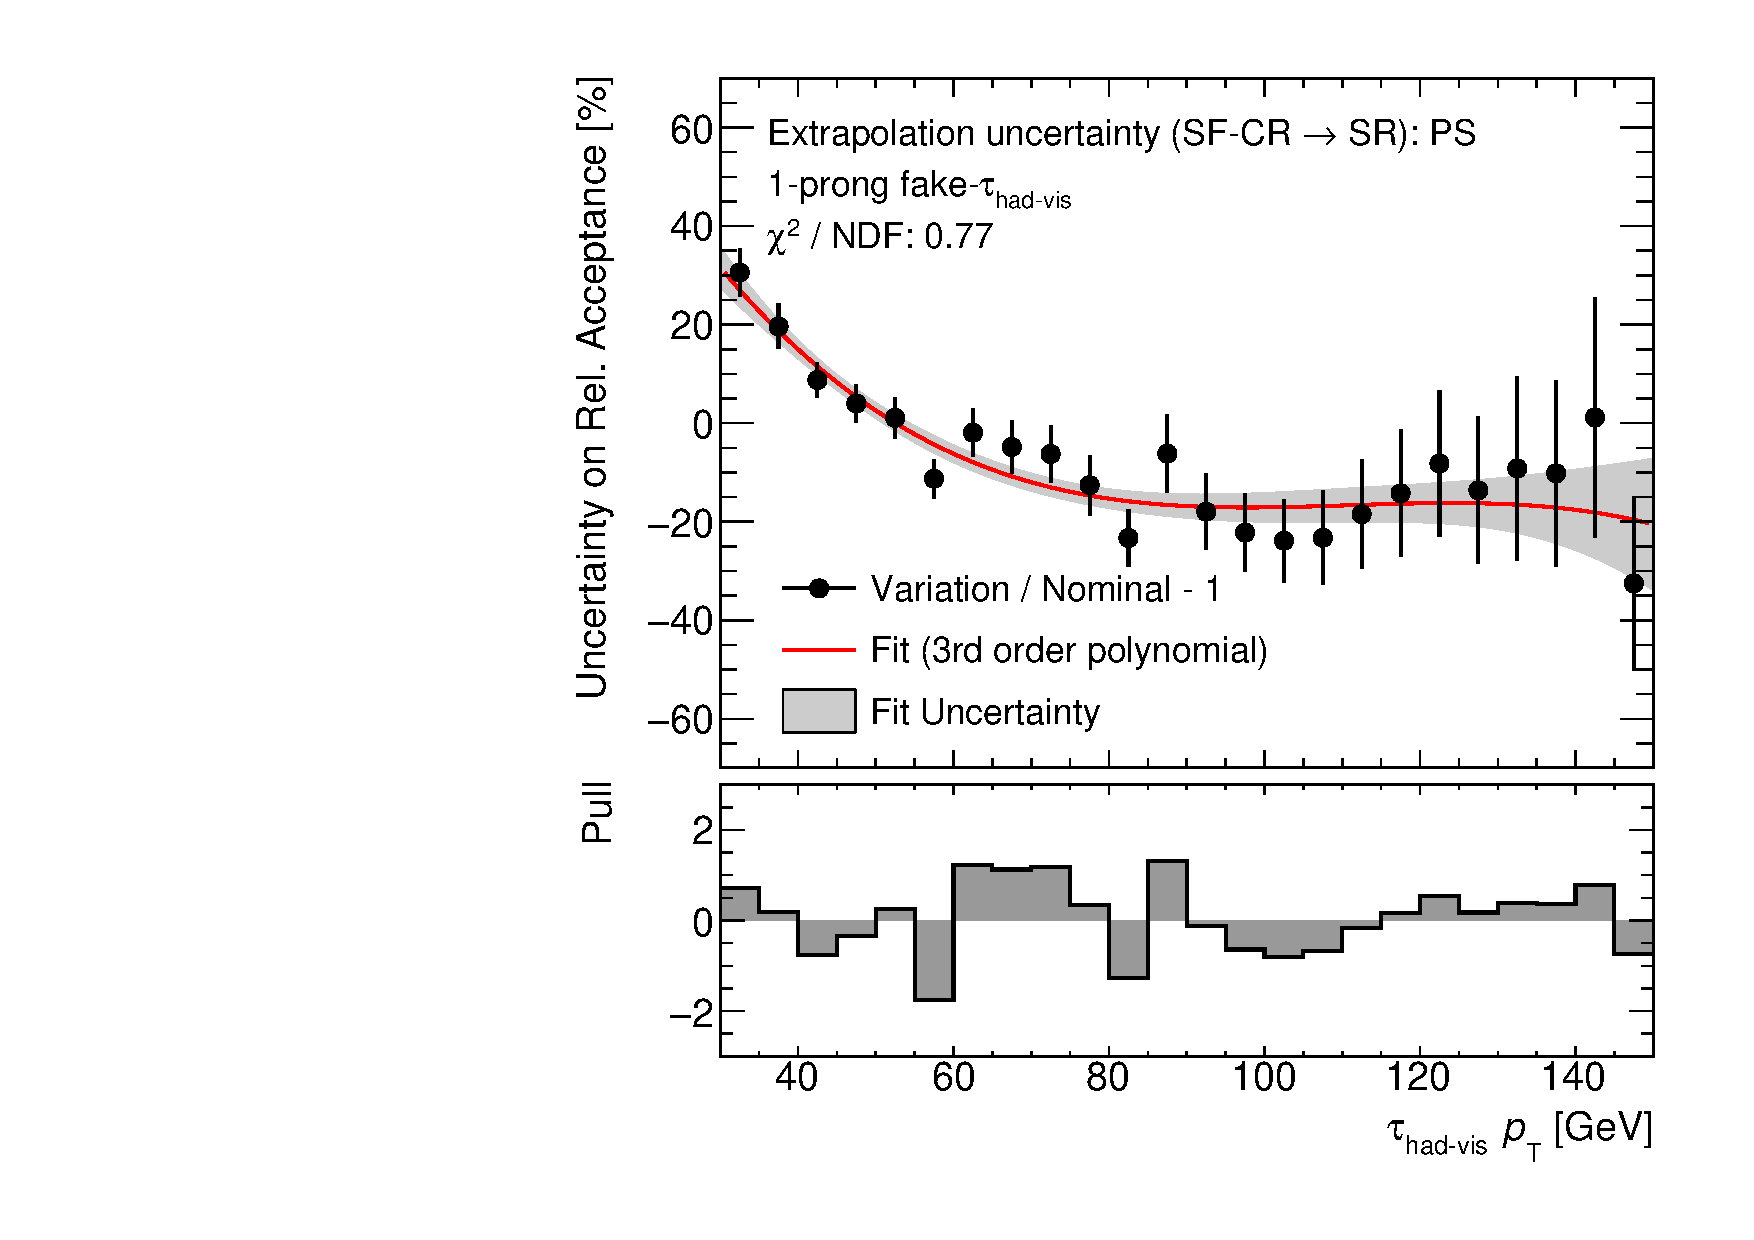
\includegraphics[width=\textwidth]{ttbarSF/ttbarSF_extrapol_PS_1p}
    \caption{}
    \label{fig:ttbarSF_extrapol_shape_a}
  \end{subfigure}\hfill%
  \begin{subfigure}[t]{.495\textwidth}
    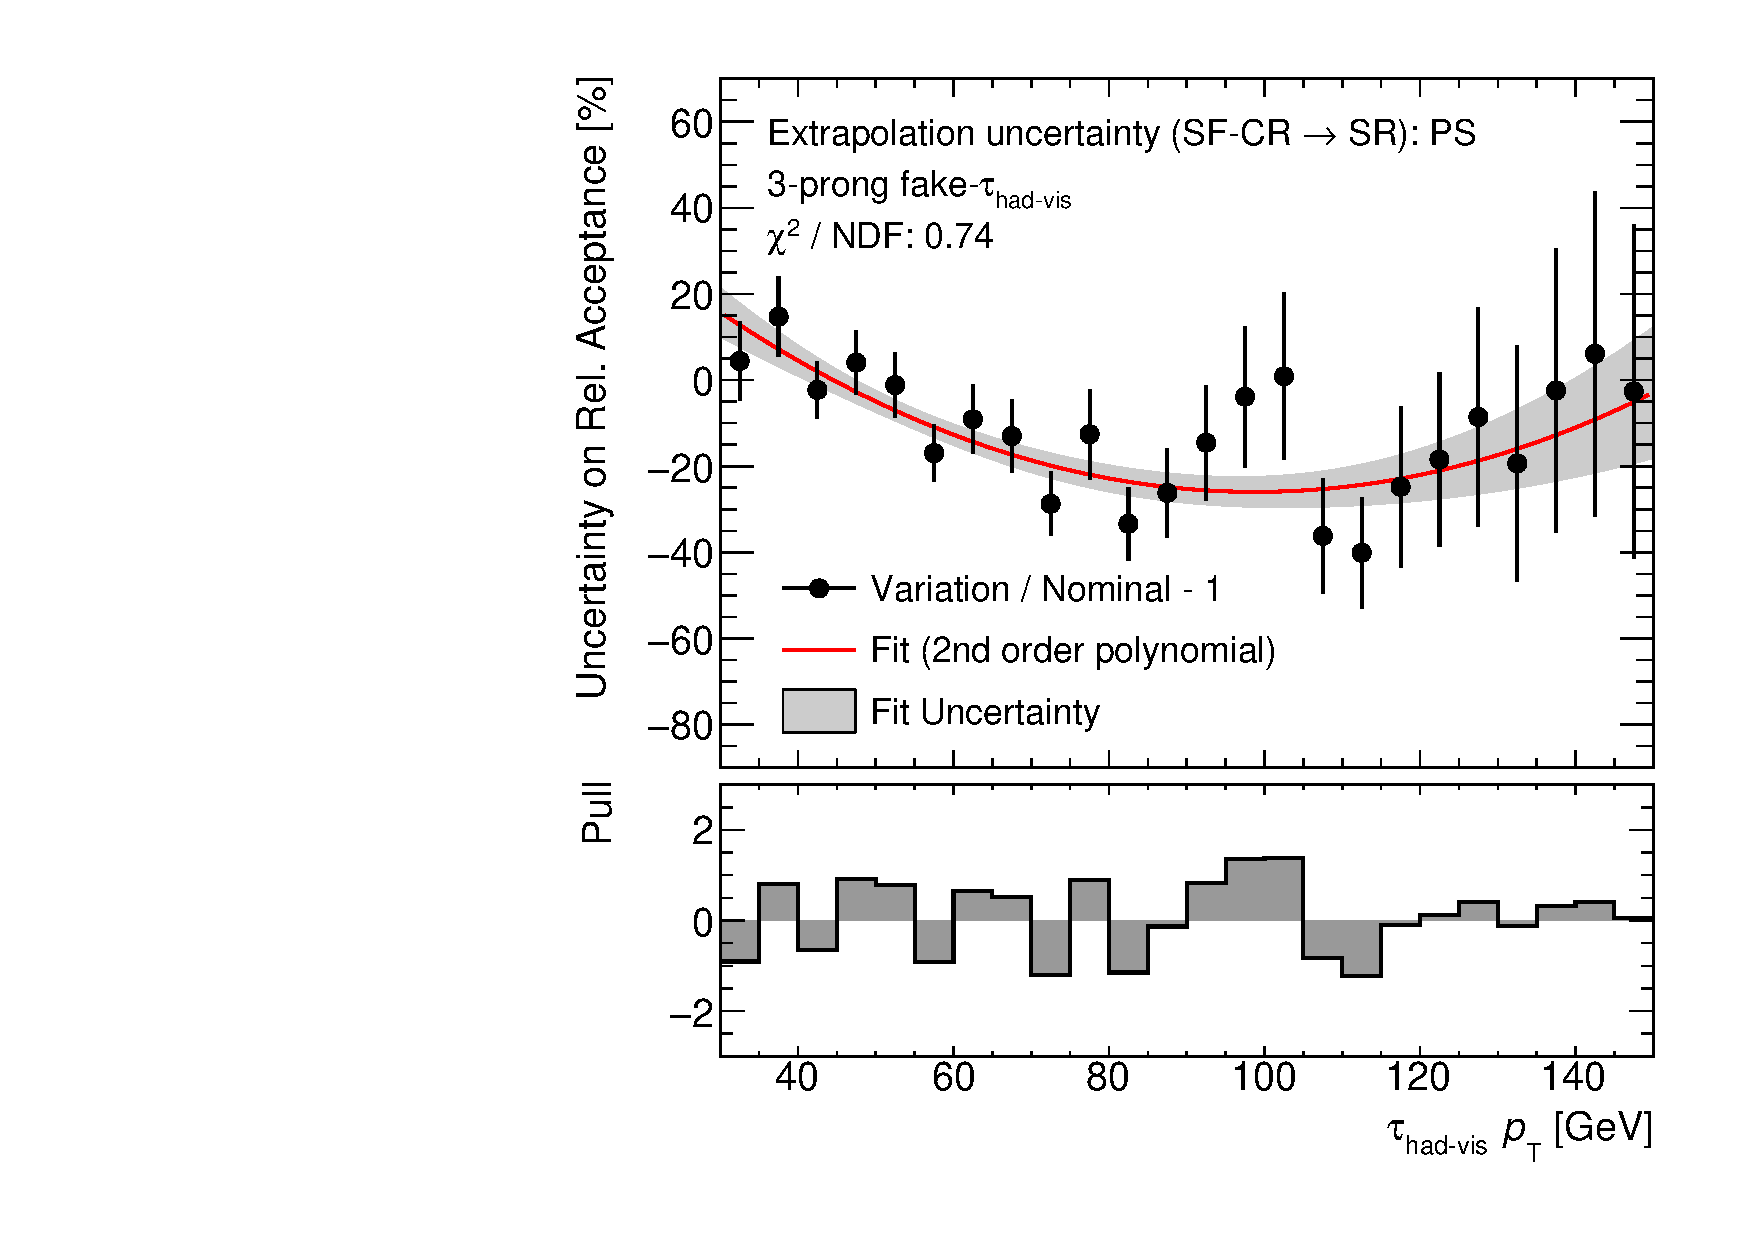
\includegraphics[width=\textwidth]{ttbarSF/ttbarSF_extrapol_PS_3p}
    \caption{}
    \label{fig:ttbarSF_extrapol_shape_b}
  \end{subfigure}

  \caption{Extrapolation uncertainty of the scale factors measured in
    the SF-CR to the \hadhad SR based on parton shower comparisons
    (\PYTHIA[8] and \HERWIG[7]). The uncertainty is shown for 1-prong
    (a) and 3-prong \faketauhadvis (b) including a fit of polynomials
    to the binned estimate of the uncertainty. }
  \label{fig:ttbarSF_extrapol_shape}
\end{figure}

A different approach is taken for the extrapolation uncertainty
between SF-CR and \hadhad SR for cases where both \tauhadvis
candidates are faked by a quark- or gluon-jet. Only a normalisation
uncertainty is assigned due to the ambiguous matching of \tauhadvis
candidates between the \lephad (1 \faketauhadvis) and the \hadhad
region (2 \faketauhadvis). This approximation is made to avoid this
ambiguity and is further motivated by it being a subdominant component
relative to the total \ttbarFakes background.

The extrapolation uncertainties are summarised
in~\Cref{tab:ttbarSF_acceptance_uncertainty}. The parton shower
variations dominate the total uncertainty on the relative acceptance
between the SF-CR and the SR, ranging from \SIrange{20}{40}{\percent}.

\begin{table}[htbp]
  \centering

  \begin{tabular}{l
  S[table-format=1.3]
  S[table-format=1.2]
  S}
  \toprule
  Source & {Uncertainty (1-prong) / \%} & {Uncertainty (3-prong) / \%} & {Uncertainty (FF) / \%} \\
  \midrule
  ME & 1.7 & 6.0 & 9.2 \\
  PS & {--$^\dagger$} & {--$^\dagger$} & 35 \\
  \hdamp & 1.6 & 8.2 & 4.6 \\
  \muF & 0.18 & 0.22 & \\
  \muR & 0.040 & 0.50 & \\
  ISR & 0.22 & 0.68 & \\
  FSR & 4.0 & 8.5 & \\
  \midrule
  Total & 4.7 & 14 & \\
  \bottomrule
\end{tabular}

%%% Local Variables:
%%% mode: latex
%%% TeX-master: "../phd_thesis"
%%% End:


  \caption{Normalisation uncertainties on the relative acceptance
    between SF-CR and SR. The uncertainties are symmetrised and
    rounded to two significant figures. $\dagger$: The parton shower
    uncertainty is parametrised as a function of \tauhadvis \pT (see
    also~\Cref{fig:ttbarSF_extrapol_shape}) and is not included in the
    total uncertainty.}
  \label{tab:ttbarSF_acceptance_uncertainty}
\end{table}


\subsubsection{Anti-ID measurement?}

This measurement was repeated in the Anti-ID region to provide an
estimate of the uncertainty of the subtraction for the fake factor
method.

\todo[inline]{Possibly include the SS region (in addition to OS) to
  get better constraints on ttbar and ttbarFakes. Possibly can float
  both true and fake \ttbar in every region reducing the correlation
  between the resulting NFs. One would have to account for possible
  biases from charge correlations.}


\todo[inline]{Fitting polynomials to the uncertainties is not well
  justified. A more general set of smooth functions should be
  considered for example by using Gaussian process regression
  instead.}

%%% Local Variables:
%%% mode: latex
%%% TeX-master: "../../phd_thesis"
%%% End:
